% Options for packages loaded elsewhere
\PassOptionsToPackage{unicode}{hyperref}
\PassOptionsToPackage{hyphens}{url}
%
\documentclass[
  11pt,
]{article}
\usepackage{amsmath,amssymb}
\usepackage{lmodern}
\usepackage{iftex}
\ifPDFTeX
  \usepackage[T1]{fontenc}
  \usepackage[utf8]{inputenc}
  \usepackage{textcomp} % provide euro and other symbols
\else % if luatex or xetex
  \usepackage{unicode-math}
  \defaultfontfeatures{Scale=MatchLowercase}
  \defaultfontfeatures[\rmfamily]{Ligatures=TeX,Scale=1}
\fi
% Use upquote if available, for straight quotes in verbatim environments
\IfFileExists{upquote.sty}{\usepackage{upquote}}{}
\IfFileExists{microtype.sty}{% use microtype if available
  \usepackage[]{microtype}
  \UseMicrotypeSet[protrusion]{basicmath} % disable protrusion for tt fonts
}{}
\makeatletter
\@ifundefined{KOMAClassName}{% if non-KOMA class
  \IfFileExists{parskip.sty}{%
    \usepackage{parskip}
  }{% else
    \setlength{\parindent}{0pt}
    \setlength{\parskip}{6pt plus 2pt minus 1pt}}
}{% if KOMA class
  \KOMAoptions{parskip=half}}
\makeatother
\usepackage{xcolor}
\IfFileExists{xurl.sty}{\usepackage{xurl}}{} % add URL line breaks if available
\IfFileExists{bookmark.sty}{\usepackage{bookmark}}{\usepackage{hyperref}}
\hypersetup{
  pdftitle={STA610 Case Study 1},
  pdfauthor={Emily Gentles (Presenter); Weiyi Liu (Writer); Jack McCarthy (Programmer); Qinzhe Wang (Coordinator \& Checker)},
  hidelinks,
  pdfcreator={LaTeX via pandoc}}
\urlstyle{same} % disable monospaced font for URLs
\usepackage[margin=1.5cm]{geometry}
\usepackage{color}
\usepackage{fancyvrb}
\newcommand{\VerbBar}{|}
\newcommand{\VERB}{\Verb[commandchars=\\\{\}]}
\DefineVerbatimEnvironment{Highlighting}{Verbatim}{commandchars=\\\{\}}
% Add ',fontsize=\small' for more characters per line
\usepackage{framed}
\definecolor{shadecolor}{RGB}{248,248,248}
\newenvironment{Shaded}{\begin{snugshade}}{\end{snugshade}}
\newcommand{\AlertTok}[1]{\textcolor[rgb]{0.94,0.16,0.16}{#1}}
\newcommand{\AnnotationTok}[1]{\textcolor[rgb]{0.56,0.35,0.01}{\textbf{\textit{#1}}}}
\newcommand{\AttributeTok}[1]{\textcolor[rgb]{0.77,0.63,0.00}{#1}}
\newcommand{\BaseNTok}[1]{\textcolor[rgb]{0.00,0.00,0.81}{#1}}
\newcommand{\BuiltInTok}[1]{#1}
\newcommand{\CharTok}[1]{\textcolor[rgb]{0.31,0.60,0.02}{#1}}
\newcommand{\CommentTok}[1]{\textcolor[rgb]{0.56,0.35,0.01}{\textit{#1}}}
\newcommand{\CommentVarTok}[1]{\textcolor[rgb]{0.56,0.35,0.01}{\textbf{\textit{#1}}}}
\newcommand{\ConstantTok}[1]{\textcolor[rgb]{0.00,0.00,0.00}{#1}}
\newcommand{\ControlFlowTok}[1]{\textcolor[rgb]{0.13,0.29,0.53}{\textbf{#1}}}
\newcommand{\DataTypeTok}[1]{\textcolor[rgb]{0.13,0.29,0.53}{#1}}
\newcommand{\DecValTok}[1]{\textcolor[rgb]{0.00,0.00,0.81}{#1}}
\newcommand{\DocumentationTok}[1]{\textcolor[rgb]{0.56,0.35,0.01}{\textbf{\textit{#1}}}}
\newcommand{\ErrorTok}[1]{\textcolor[rgb]{0.64,0.00,0.00}{\textbf{#1}}}
\newcommand{\ExtensionTok}[1]{#1}
\newcommand{\FloatTok}[1]{\textcolor[rgb]{0.00,0.00,0.81}{#1}}
\newcommand{\FunctionTok}[1]{\textcolor[rgb]{0.00,0.00,0.00}{#1}}
\newcommand{\ImportTok}[1]{#1}
\newcommand{\InformationTok}[1]{\textcolor[rgb]{0.56,0.35,0.01}{\textbf{\textit{#1}}}}
\newcommand{\KeywordTok}[1]{\textcolor[rgb]{0.13,0.29,0.53}{\textbf{#1}}}
\newcommand{\NormalTok}[1]{#1}
\newcommand{\OperatorTok}[1]{\textcolor[rgb]{0.81,0.36,0.00}{\textbf{#1}}}
\newcommand{\OtherTok}[1]{\textcolor[rgb]{0.56,0.35,0.01}{#1}}
\newcommand{\PreprocessorTok}[1]{\textcolor[rgb]{0.56,0.35,0.01}{\textit{#1}}}
\newcommand{\RegionMarkerTok}[1]{#1}
\newcommand{\SpecialCharTok}[1]{\textcolor[rgb]{0.00,0.00,0.00}{#1}}
\newcommand{\SpecialStringTok}[1]{\textcolor[rgb]{0.31,0.60,0.02}{#1}}
\newcommand{\StringTok}[1]{\textcolor[rgb]{0.31,0.60,0.02}{#1}}
\newcommand{\VariableTok}[1]{\textcolor[rgb]{0.00,0.00,0.00}{#1}}
\newcommand{\VerbatimStringTok}[1]{\textcolor[rgb]{0.31,0.60,0.02}{#1}}
\newcommand{\WarningTok}[1]{\textcolor[rgb]{0.56,0.35,0.01}{\textbf{\textit{#1}}}}
\usepackage{graphicx}
\makeatletter
\def\maxwidth{\ifdim\Gin@nat@width>\linewidth\linewidth\else\Gin@nat@width\fi}
\def\maxheight{\ifdim\Gin@nat@height>\textheight\textheight\else\Gin@nat@height\fi}
\makeatother
% Scale images if necessary, so that they will not overflow the page
% margins by default, and it is still possible to overwrite the defaults
% using explicit options in \includegraphics[width, height, ...]{}
\setkeys{Gin}{width=\maxwidth,height=\maxheight,keepaspectratio}
% Set default figure placement to htbp
\makeatletter
\def\fps@figure{htbp}
\makeatother
\setlength{\emergencystretch}{3em} % prevent overfull lines
\providecommand{\tightlist}{%
  \setlength{\itemsep}{0pt}\setlength{\parskip}{0pt}}
\setcounter{secnumdepth}{-\maxdimen} % remove section numbering
\usepackage{booktabs}
\usepackage{longtable}
\usepackage{array}
\usepackage{multirow}
\usepackage{wrapfig}
\usepackage{float}
\usepackage{colortbl}
\usepackage{pdflscape}
\usepackage{tabu}
\usepackage{threeparttable}
\usepackage{threeparttablex}
\usepackage[normalem]{ulem}
\usepackage{makecell}
\usepackage{xcolor}
\ifLuaTeX
  \usepackage{selnolig}  % disable illegal ligatures
\fi

\title{STA610 Case Study 1}
\author{Emily Gentles (Presenter) \and Weiyi Liu (Writer) \and Jack
McCarthy (Programmer) \and Qinzhe Wang (Coordinator \& Checker)}
\date{15 October, 2021}

\begin{document}
\maketitle

\hypertarget{introduction}{%
\section{Introduction}\label{introduction}}

Prescription opioid abuse has recently become an epidemic in the United
States. The price of illicit prescription opioids indicates the
supply-demand relationship of the drug. This case study aims to explore
the relationship between the unit price of drugs and other factors such
as the quantity purchased, the location of the transaction, and strength
of the drug. More specifically, our group's interest is to explore the
factors related to the cost per milligram and the heterogeneity in the
region. The dataset we will be using is provided by StreetRx, a
reporting tool for people at large to anonymously report the price they
paid or heard for diverted prescription drugs.

Our drug of interest is Morphine which is used to ``relieve moderate to
severe pain and may be habit-forming,'' especially with prolonged use
(MedlinePlus).

\hypertarget{eda}{%
\section{EDA}\label{eda}}

\hypertarget{missing-values}{%
\subsubsection{Missing Values}\label{missing-values}}

The subset of the StreetRx dataset pertaining to Morphine contains 9,268
observations with 13 variables. There are 13,443 empty cells, including
both missing values and blank entries. To maintain the statistical power
and avoid bias, our group decided to recode both the empty cells and ``0
Reporter did not answer this question'' in \texttt{Primary\_Reason}
(5061 in total) as ``8 Prefer not to answer'' and recode the empty cells
in \texttt{source} (3942 in total) as ``Blank'' because of the high
missing rates. Then, we removed other rows with missing values.

Additionally, we removed non-positive price values as well as price
values greater than 10. Since the data is self-reported, these extremely
expensive prices are likely due to users misunderstanding the system and
reporting total price instead of unit price. The number of observations
is now 5,582.

\hypertarget{response-variable-price-per-milligram}{%
\subsubsection{Response Variable: Price per
milligram}\label{response-variable-price-per-milligram}}

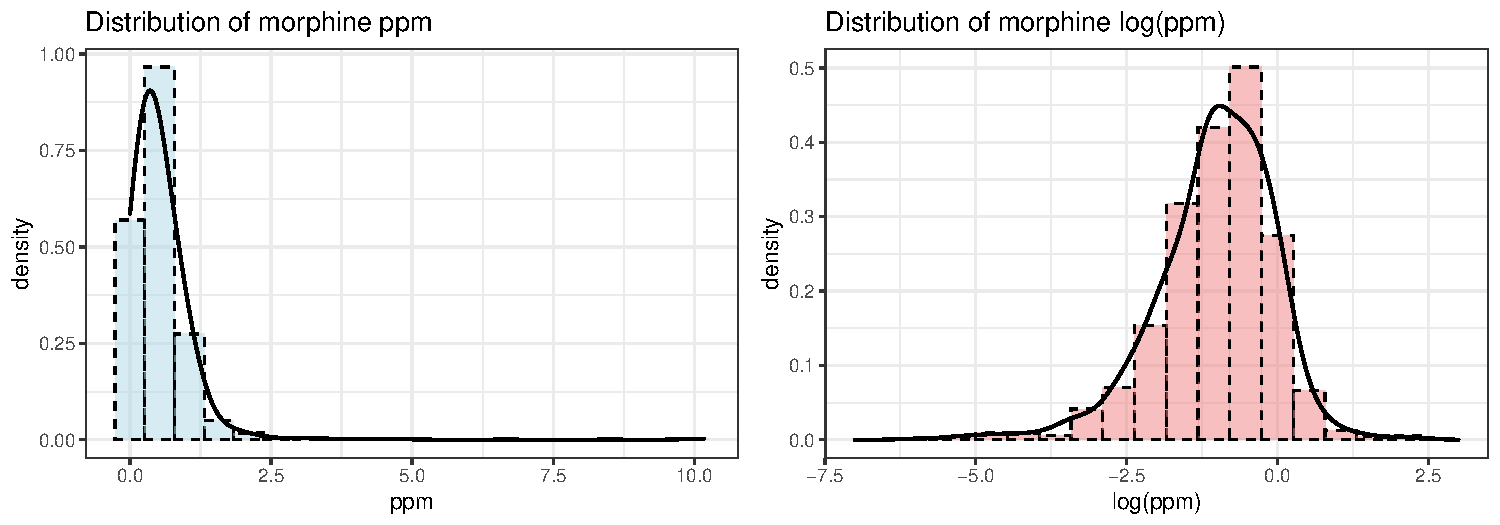
\includegraphics{cs1_files/figure-latex/unnamed-chunk-4-1.pdf}

Whether we fit a hierarchical model or linear regression, the response
variable should be normally distributed. Although the normality
assumption pertains to the conditional distribution of our response
variable, it's still beneficial to check the assumption for the marginal
distribution as a very skewed marginal distribution could persist and
affect the model's resulting conditional distribution. From the
histogram on the left, the distribution of \texttt{ppm} is clearly
right-skewed. Since \texttt{ppm} is strictly non-negative, a log
transformation may be appropriate. We can see that the distribution of
\texttt{log(ppm)}, given above, appears to be much closer to the desired
normal distribution.

\hypertarget{grouping-variable-city-state-and-usa_region}{%
\subsubsection{Grouping Variable: city, state, and
USA\_region}\label{grouping-variable-city-state-and-usa_region}}

Since we want to analyze the heterogeneity in pricing by location, we
have three choices of grouping variables, \texttt{city}, \texttt{state},
and \texttt{USA\_region}.

\textbf{City}

There are 1642 unique \texttt{city} values, and many cities have small
sample size (i.e.~less than 5 observations). We decide not to use
\texttt{city} as the grouping variable (see appendix).

\textbf{State}

As for the state, we examined the sample sizes in each group and decided
to out filter Puerto Rico and Vermont because they have less than 5
observations.

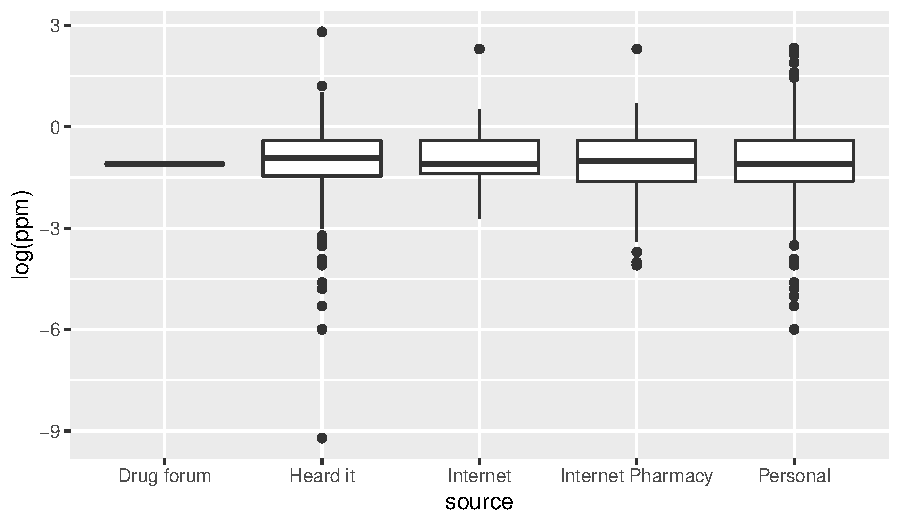
\includegraphics{cs1_files/figure-latex/unnamed-chunk-8-1.pdf}

We then inspect the state-level differences more closely by plotting the
group-level means against the sample sizes. We observed that the
within-state means for states with smaller sample sizes vary a lot,
while the within-state means for states with higher sample sizes in
general adhere more closely to the grand mean. This is conducive to the
borrowing of information between states with a hierarchical model. From
the above boxplot of \texttt{log(ppm)} against \texttt{state}, it is
also evident that the \texttt{log(ppm)} distributions differ across
states. This indicates the potential state-level differences in drug
prices. Therefore, we decide to use state as our grouping variable at
this stage.

\textbf{Region}

From the boxplot we see that the \texttt{log(ppm)} distributions differ
slightly across regions, though not as much as across states. We may
also consider using region as the grouping variable.

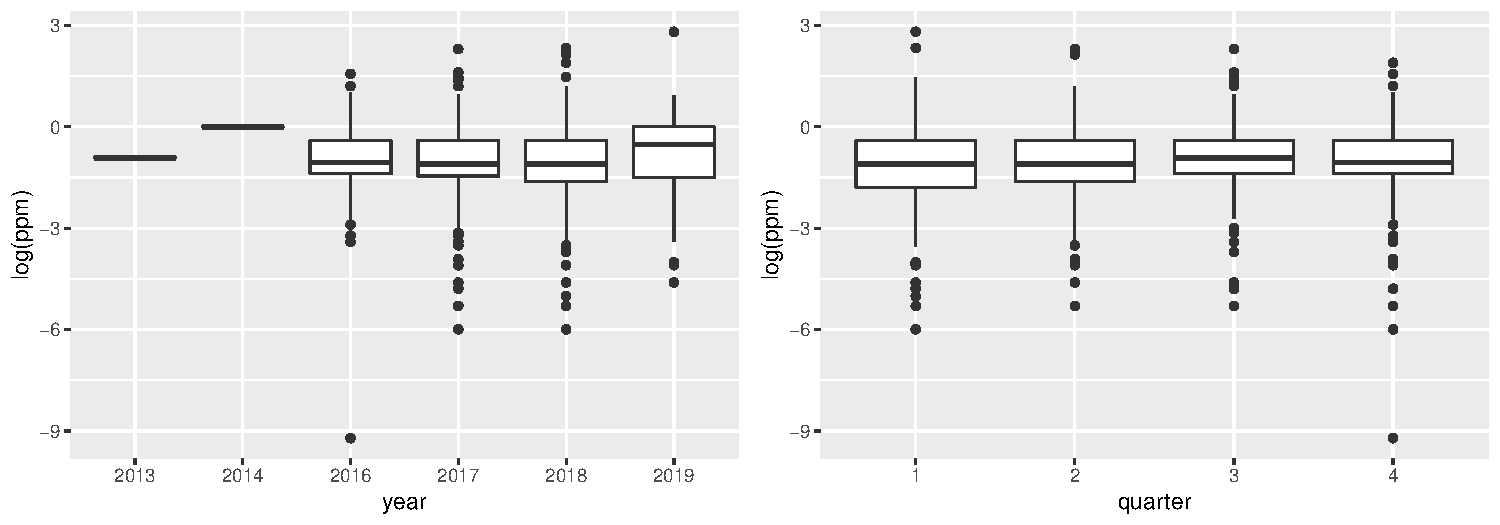
\includegraphics{cs1_files/figure-latex/unnamed-chunk-9-1.pdf}

\hypertarget{date-price_date}{%
\subsubsection{Date (price\_date)}\label{date-price_date}}

As for the \texttt{price\_date}, we noticed some observations are prior
to the establishment of StreetRx, which are likely incorrect inputs. We
dropped the observations before 2010. For the remaining observations, we
came up with two ways of data cleaning. The first choice is to choose a
starting date and convert the feature as the date differences
(\texttt{date\_diff}) from that starting date. The second choice is to
split this date variable into two components, \texttt{year} and
\texttt{quarter}, to explore the trend of unit drug price over time and
the seasonality.

Our visualizations suggested there is no clear indication that the log
value of per milligram price of morphine varies along with
\texttt{date\_diff}. However, for different \texttt{year} and
\texttt{quarter}, the \texttt{log(ppm)} value varies slightly (see
appendix).

\hypertarget{bulk_purchase-source}{%
\subsubsection{Bulk\_purchase \& Source}\label{bulk_purchase-source}}

\includegraphics{cs1_files/figure-latex/unnamed-chunk-16-1.pdf}

There is no need to conduct any data cleaning on
\texttt{bulk\_purchase}. And from the boxplot (see appendix), there is a
slight trend that the drug price may be lower if purchased in bulk.
Therefore, \texttt{bulk\_purchase} might be a potential predictor.

For the feature \texttt{source}, we have recoded the missing value as
``Blank'' and the name of websites as ``Internet''. We also dropped the
only observation whose \texttt{source} is ``Drug Forum''. The boxplot
shows that the \texttt{log(ppm)} value varies among different sources
(see appendix).

\hypertarget{dosage-strength-primary-reason}{%
\subsubsection{Dosage Strength \& Primary
Reason}\label{dosage-strength-primary-reason}}

\includegraphics{cs1_files/figure-latex/unnamed-chunk-20-1.pdf}

From the scatter plot of \texttt{log(ppm)} against \texttt{mgstr}, there
is a slight trend that the larger the dosage strength, the smaller the
per milligram price. We have also noticed that \texttt{mgstr} only takes
16 discrete values. Therefore, we decided to transform it into 4 levels
(``low'', ``medium'', ``medium high'', and ``high'') based on the 0.25,
0.5, and 0.75 quantiles of \texttt{mgstr}. From the boxplot, the trend
that the \texttt{log(ppm)} values decrease as the dosage strength
increases is more clear when using these new levels.

For \texttt{primary\_reason}, we have converted the empty cells and ``0
Reporter did not answer this question'' to ``8 Prefer not to answer''.
The \texttt{log(ppm)} value varies among different reasons for
purchasing morphine (see appendix).

\hypertarget{model}{%
\section{Model}\label{model}}

\hypertarget{initial-model-model-selection}{%
\subsubsection{Initial Model \& Model
Selection}\label{initial-model-model-selection}}

The goal of our analysis is to investigate factors related to the per
milligram price of morphine and explore heterogeneity in pricing by
location. As discussed in the EDA part, we do not have enough data to
estimate the effects at the city level. Meanwhile, the drug prices do
not seem to change significantly across regions. Thus, the state
variable is a preferable choice of accounting for location. Since many
states have relatively small sample sizes, a hierarchical model allows
us to borrow information across states.

Comparing three full models with different grouping variables, the AIC
and BIC score also suggest choosing \texttt{state} as the group-level
variable.

\begin{tabular}{l|r|r}
\hline
Grouping & AIC & BIC\\
\hline
City & 15408.58 & 15428.46\\
\hline
State & 15354.88 & 15374.76\\
\hline
Region & 15400.48 & 15420.36\\
\hline
\end{tabular}

Our baseline model incorporates only the state-level random intercepts.
For other individual-level predictors, we add one variable to the model
each time and use both the Likelihood Ratio test and the BIC score to
determine whether it should be added. The \textbf{LRT} is designed for
nested models while the BIC score considers both the likelihood and the
model complexity and gives a more general sense of model performance.
The table below displays the results of model selection. We also used
the full model as a starting point to perform stepwise backward
elimination with the results agreeing the previous model selection
method. (See appendix).

Our final model incorporates the grouping variable \texttt{state} and
the individual level predictors \texttt{mgstr} (recoded as 4 levels), as
well as \texttt{bulk\_purchase}, \texttt{quarter}, and \texttt{source}.

\begin{table}[!h]
\centering
\begin{tabular}{l|l|r}
\hline
Model & LRT.p.value & BIC\\
\hline
\cellcolor{gray!6}{(1|state)} & \cellcolor{gray!6}{} & \cellcolor{gray!6}{15374.76}\\
\hline
(1|state) + mgstr2 & 0 & 14615.63\\
\hline
\cellcolor{gray!6}{(1|state) + mgstr2 + bulk\_purchase} & \cellcolor{gray!6}{2e-04} & \cellcolor{gray!6}{14610.01}\\
\hline
(1|state) + mgstr2 + bulk\_purchase + year & 0.1079 & 14673.21\\
\hline
\cellcolor{gray!6}{(1|state) + mgstr2 + bulk\_purchase + quarter} & \cellcolor{gray!6}{0.0213} & \cellcolor{gray!6}{14626.19}\\
\hline
(1|state) + mgstr2 + bulk\_purchase + date\_diff & 0.1844 & 14616.87\\
\hline
\cellcolor{gray!6}{(1|state) + mgstr2 + bulk\_purchase + quarter + source} & \cellcolor{gray!6}{7e-04} & \cellcolor{gray!6}{14641.45}\\
\hline
(1|state) + mgstr2 + bulk\_purchase + quarter + source + primary\_reason & 1 & 14681.42\\
\hline
\end{tabular}
\end{table}

\hypertarget{interactions}{%
\subsubsection{Interactions}\label{interactions}}

To be added, all codes are in appendix, no interaction term can improve
the model performance.

\hypertarget{final-model}{%
\subsubsection{Final Model}\label{final-model}}

Our final model is
\[log(y_{ij}) = \beta_0 + b_{0j} + \beta_1 M_{ij} + \beta_2 B_{ij} + \beta_3 Q_{ij} + \beta_4 S_{ij} + \epsilon_{ij}\]
\[b_{0j} \sim \mathcal{N}(0, \tau^2) \perp \epsilon_{ij} \stackrel{iid} \sim \mathcal{N}(0, \sigma^2)\]
The response variable and predictors are defined as:

\begin{itemize}
\item
  \(y_ij\): Per milligram price of morphine for individual i in state j
\item
  \(M_{ij}\): Dosage strength in mg of the units purchased, factored
  into 4 levels
\item
  \(B_{ij}\): Bulk purchase, an indicator for whether 10+ units were
  purchased at once
\item
  \(Q_{ij}\): Quarter of the reported purchase
\item
  \(S_{ij}\): Source of information (including first-hand and
  second-hand sources)
\end{itemize}

\hypertarget{model-diagnostics}{%
\subsubsection{Model Diagnostics}\label{model-diagnostics}}

\includegraphics{cs1_files/figure-latex/unnamed-chunk-29-1.pdf}

\begin{itemize}
\tightlist
\item
  \texttt{Residual\ vs.\ Fitted\ plot}: The residuals are spread equally
  around the horizontal line, indicating there is no non-linear
  relationship.
\item
  \texttt{Normal\ QQ\ plot\ for\ residuals}: The normality assumption is
  slightly met since our residuals adhere around the diagonal line
  representing normality but have heavy tails on both sides. We also
  have one data point that deviates severely from the diagonal line.
\item
  \texttt{Normal\ QQ\ plot\ for\ Random\ Effects}: We can accept the
  random effects are normally distributed. But we still have three
  outliers.
\item
  \texttt{Cook\textquotesingle{}s\ Distance}: We have 3 highly
  influential states (Florida, Pennsylvania, and California) whose
  Cook's distance exceeds the \(\frac{4}{n}\) cutoff, where n denotes
  the number of states.
\end{itemize}

We tried to remove the data point with the lowest residual and the
influential groups to address the violated assumptions. However, this
did not drastically improve the normality of the residuals (see
appendix). Moreover, the influential states have a considerable sample
size (1382 observations). Therefore, we decide only to drop the
individual level outlier but keep all the groups.

\includegraphics{cs1_files/figure-latex/unnamed-chunk-30-1.pdf}

To be added, no significant improvement

\hypertarget{conclusion}{%
\section{Conclusion}\label{conclusion}}

\hypertarget{fixed-effects}{%
\subsubsection{Fixed Effects}\label{fixed-effects}}

\begin{table}[!h]
\centering
\begin{tabular}{l|r|r|r|r|r|r}
\hline
  & Estimate & exp(Estimate) & Std. Error & df & t value & Pr(>|t|)\\
\hline
\cellcolor{gray!6}{(Intercept)} & \cellcolor{gray!6}{-0.6346} & \cellcolor{gray!6}{0.5301} & \cellcolor{gray!6}{0.0393} & \cellcolor{gray!6}{296.1819} & \cellcolor{gray!6}{-16.1290} & \cellcolor{gray!6}{0.0000}\\
\hline
quarter2 & 0.0854 & 1.0891 & 0.0321 & 5550.5948 & 2.6578 & 0.0079\\
\hline
\cellcolor{gray!6}{quarter3} & \cellcolor{gray!6}{0.0841} & \cellcolor{gray!6}{1.0877} & \cellcolor{gray!6}{0.0332} & \cellcolor{gray!6}{5555.0726} & \cellcolor{gray!6}{2.5349} & \cellcolor{gray!6}{0.0113}\\
\hline
quarter4 & 0.0844 & 1.0881 & 0.0341 & 5551.1650 & 2.4759 & 0.0133\\
\hline
\cellcolor{gray!6}{sourceHeard it} & \cellcolor{gray!6}{0.0633} & \cellcolor{gray!6}{1.0653} & \cellcolor{gray!6}{0.0335} & \cellcolor{gray!6}{5556.1197} & \cellcolor{gray!6}{1.8904} & \cellcolor{gray!6}{0.0588}\\
\hline
sourceInternet & -0.0041 & 0.9959 & 0.0625 & 5555.5822 & -0.0656 & 0.9477\\
\hline
\cellcolor{gray!6}{sourceInternet Pharmacy} & \cellcolor{gray!6}{-0.3227} & \cellcolor{gray!6}{0.7242} & \cellcolor{gray!6}{0.1016} & \cellcolor{gray!6}{5548.9347} & \cellcolor{gray!6}{-3.1743} & \cellcolor{gray!6}{0.0015}\\
\hline
sourcePersonal & -0.0398 & 0.9609 & 0.0281 & 5557.7473 & -1.4157 & 0.1569\\
\hline
\cellcolor{gray!6}{mgstr22 medium} & \cellcolor{gray!6}{-0.3816} & \cellcolor{gray!6}{0.6827} & \cellcolor{gray!6}{0.0279} & \cellcolor{gray!6}{5549.1951} & \cellcolor{gray!6}{-13.6631} & \cellcolor{gray!6}{0.0000}\\
\hline
mgstr23 medium high & -0.7000 & 0.4966 & 0.0365 & 5554.7006 & -19.1836 & 0.0000\\
\hline
\cellcolor{gray!6}{mgstr24 high} & \cellcolor{gray!6}{-1.1197} & \cellcolor{gray!6}{0.3264} & \cellcolor{gray!6}{0.0420} & \cellcolor{gray!6}{5559.7107} & \cellcolor{gray!6}{-26.6889} & \cellcolor{gray!6}{0.0000}\\
\hline
bulk\_purchase1 Bulk purchase & -0.1141 & 0.8922 & 0.0296 & 5557.9880 & -3.8488 & 0.0001\\
\hline
\end{tabular}
\end{table}

\begin{itemize}
\item
  Quarter (baseline: Quarter1): Compared with quarter 1, holding all
  other predictors unchanged, purchasing the morphine in quarter 2, the
  per milligram price of the drug will increase by a multiplicative
  effect of \(e^{0.0853} = 1.0891\) (about 8.91\%). Similarly, if the
  drug is purchased in quarter 3 or 4, the drug price will increase by
  8.77\% and 8.81\%, respectively.
\item
  Source (baseline: Blank): Compared with an unknown source, holding all
  other predictors unchanged, the per milligram drug price heard from
  other people will increase by a multiplicative effect of
  \(e^{0.0633} = 1.0653\) (about 6.53\%). Similarly, the price
  information obtained from the internet, internet pharmacy, or personal
  purchase will decrease by 0.41\%, 27.58\%, and 3.91\%, respectively.
\item
  Dosage Strength (baseline: Low): Compared with low dosage strength,
  holding all other predictors unchanged, the per milligram price of
  morphine will decrease by a multiplicative effect of
  \(e^{-0.3816} = 0.6827\) (about 31.73\%) if it has medium dosage
  strength. Similarly, if the dosage strength is medium-high or high,
  the drug price will decrease by 50.34\% and 67.36\%, respectively.
\item
  Bulk Purchase (baseline: Not bulk purchase): Compared with non-bulk
  purchase, holding all other predictors unchanged, the unit price of
  morphine will decrease by a multiplicative effect of
  \(e^{0.1141} = 0.8922\) (about 10.78\%).
\end{itemize}

\hypertarget{random-effects}{%
\subsubsection{Random Effects}\label{random-effects}}

\begin{table}[!h]
\centering
\begin{tabular}{l|r|r}
\hline
  & $\tau^2$ & $\sigma^2$\\
\hline
\cellcolor{gray!6}{Estimate} & \cellcolor{gray!6}{0.0161} & \cellcolor{gray!6}{0.7772}\\
\hline
\end{tabular}
\end{table}

The estimated across-state variance is \(\hat{\tau^2} = 0.0161\), which
also describes the variation attributed to the random intercept. The
estimated within-state variance is \(\hat{\sigma^2} = 0.7772\), which
describes the unexplained variation. The estimated interclass
correlation is
\(\frac{\hat{\tau^2}}{\hat{\tau^2} + \hat{\sigma^2}} \approx 0.02\).
Therefore, we have little correlation within the same state.

\includegraphics{cs1_files/figure-latex/unnamed-chunk-37-1.pdf}

From the random intercepts plot, we can see that states have different
bases per milligram morphine prices. The prices ranges from
\(e^{-0.2297} = 0.7948\) (Michigan) to \(e^{0.2063} = 1.2292\)
(Massachusetts). These estimates are based on the baseline condition of
all other predictors, which are purchasing in quarter 1, from an unknown
source, with low dosage strength, and not purchased in bulk

\hypertarget{limitation}{%
\section{Limitation}\label{limitation}}

\newpage

\hypertarget{appendix}{%
\section{Appendix}\label{appendix}}

\begin{Shaded}
\begin{Highlighting}[]
\CommentTok{\# knitr::opts\_chunk$set(warning=FALSE, message = FALSE, cache = TRUE)}
\FunctionTok{library}\NormalTok{(tidyverse)}
\FunctionTok{library}\NormalTok{(janitor)}
\FunctionTok{library}\NormalTok{(gridExtra)}
\FunctionTok{library}\NormalTok{(cowplot)}
\FunctionTok{library}\NormalTok{(knitr)}
\FunctionTok{require}\NormalTok{(magrittr)}
\FunctionTok{require}\NormalTok{(dplyr)}
\FunctionTok{library}\NormalTok{(kableExtra)}
\FunctionTok{library}\NormalTok{(readr)}
\FunctionTok{library}\NormalTok{(tidyr)}
\FunctionTok{library}\NormalTok{(broom)}
\FunctionTok{library}\NormalTok{(lme4)}
\FunctionTok{library}\NormalTok{(glmmTMB)}
\FunctionTok{library}\NormalTok{(sjPlot)}
\FunctionTok{library}\NormalTok{(brms)}
\FunctionTok{library}\NormalTok{(coda)}
\FunctionTok{library}\NormalTok{(rstan)}
\FunctionTok{library}\NormalTok{(tidybayes)}
\FunctionTok{library}\NormalTok{(naniar)}
\FunctionTok{library}\NormalTok{(olsrr)}
\FunctionTok{library}\NormalTok{(lmerTest)}
\FunctionTok{require}\NormalTok{(lattice)}

\CommentTok{\# devtools::install\_github("goodekat/redres")}
\FunctionTok{library}\NormalTok{(redres)}
\end{Highlighting}
\end{Shaded}

\begin{Shaded}
\begin{Highlighting}[]
\FunctionTok{load}\NormalTok{(}\StringTok{\textquotesingle{}streetrx.RData\textquotesingle{}}\NormalTok{)}
\end{Highlighting}
\end{Shaded}

\begin{Shaded}
\begin{Highlighting}[]
\NormalTok{na\_check }\OtherTok{\textless{}{-}}\NormalTok{ streetrx }\SpecialCharTok{\%\textgreater{}\%}
  \FunctionTok{filter}\NormalTok{(api\_temp }\SpecialCharTok{==} \StringTok{\textquotesingle{}morphine\textquotesingle{}}\NormalTok{) }\SpecialCharTok{\%\textgreater{}\%}
  \FunctionTok{mutate\_all}\NormalTok{( }\FunctionTok{list}\NormalTok{( }\SpecialCharTok{\textasciitilde{}}\FunctionTok{na\_if}\NormalTok{(., }\StringTok{\textquotesingle{}\textquotesingle{}}\NormalTok{) ) ) }\SpecialCharTok{\%\textgreater{}\%}
  \FunctionTok{droplevels}\NormalTok{()}

\FunctionTok{dim}\NormalTok{(na\_check)}
\FunctionTok{sum}\NormalTok{(}\FunctionTok{is.na}\NormalTok{(na\_check))}

\FunctionTok{sum}\NormalTok{(}\FunctionTok{is.na}\NormalTok{(na\_check}\SpecialCharTok{$}\NormalTok{Primary\_Reason))}

\FunctionTok{sum}\NormalTok{(}\FunctionTok{is.na}\NormalTok{(na\_check}\SpecialCharTok{$}\NormalTok{source))}

\FunctionTok{sum}\NormalTok{(}\FunctionTok{is.na}\NormalTok{(na\_check))}

\FunctionTok{gg\_miss\_upset}\NormalTok{(na\_check)}
\end{Highlighting}
\end{Shaded}

\begin{Shaded}
\begin{Highlighting}[]
\CommentTok{\# subset for group drug}

\NormalTok{morph\_data }\OtherTok{\textless{}{-}}\NormalTok{ streetrx }\SpecialCharTok{\%\textgreater{}\%}
  \FunctionTok{filter}\NormalTok{(api\_temp }\SpecialCharTok{==} \StringTok{\textquotesingle{}morphine\textquotesingle{}}\NormalTok{)}

\NormalTok{morph\_data}\SpecialCharTok{$}\NormalTok{Primary\_Reason }\OtherTok{\textless{}{-}} \FunctionTok{droplevels}\NormalTok{(morph\_data}\SpecialCharTok{$}\NormalTok{Primary\_Reason)}
\FunctionTok{levels}\NormalTok{(morph\_data}\SpecialCharTok{$}\NormalTok{Primary\_Reason)[}\DecValTok{1}\NormalTok{] }\OtherTok{\textless{}{-}} \StringTok{"8 Prefer not to answer"}
\FunctionTok{levels}\NormalTok{(morph\_data}\SpecialCharTok{$}\NormalTok{Primary\_Reason)[}\DecValTok{2}\NormalTok{] }\OtherTok{\textless{}{-}} \StringTok{"8 Prefer not to answer"}

\NormalTok{morph\_data}\SpecialCharTok{$}\NormalTok{source }\OtherTok{\textless{}{-}} \FunctionTok{droplevels}\NormalTok{(morph\_data}\SpecialCharTok{$}\NormalTok{source)}
\FunctionTok{levels}\NormalTok{(morph\_data}\SpecialCharTok{$}\NormalTok{source)[}\DecValTok{1}\NormalTok{] }\OtherTok{\textless{}{-}} \StringTok{"Blank"}

\NormalTok{morph\_data }\OtherTok{\textless{}{-}}\NormalTok{ morph\_data }\SpecialCharTok{\%\textgreater{}\%} 
  \FunctionTok{filter}\NormalTok{(}\FunctionTok{between}\NormalTok{(ppm, }\FloatTok{0.000001}\NormalTok{, }\DecValTok{10}\NormalTok{)) }\SpecialCharTok{\%\textgreater{}\%}
  \FunctionTok{mutate\_all}\NormalTok{( }\FunctionTok{list}\NormalTok{( }\SpecialCharTok{\textasciitilde{}}\FunctionTok{na\_if}\NormalTok{(., }\StringTok{\textquotesingle{}\textquotesingle{}}\NormalTok{) ) ) }\SpecialCharTok{\%\textgreater{}\%}
  \FunctionTok{drop\_na}\NormalTok{() }\SpecialCharTok{\%\textgreater{}\%}
  \FunctionTok{clean\_names}\NormalTok{() }\SpecialCharTok{\%\textgreater{}\%}
  \FunctionTok{mutate}\NormalTok{(}
    \AttributeTok{quarter=}\FunctionTok{substring}\NormalTok{(yq\_pdate, }\DecValTok{5}\NormalTok{, }\DecValTok{5}\NormalTok{),}
    \AttributeTok{year=}\FunctionTok{substring}\NormalTok{(yq\_pdate, }\DecValTok{1}\NormalTok{, }\DecValTok{4}\NormalTok{),}
    \AttributeTok{state=}\FunctionTok{recode\_factor}\NormalTok{(}\FunctionTok{droplevels}\NormalTok{(state), }\StringTok{\textquotesingle{}USA\textquotesingle{}}\OtherTok{=}\StringTok{\textquotesingle{}Unknown\textquotesingle{}}\NormalTok{)}
\NormalTok{  ) }

\FunctionTok{nrow}\NormalTok{(morph\_data)}

\FunctionTok{sum}\NormalTok{(morph\_data}\SpecialCharTok{$}\NormalTok{ppm }\SpecialCharTok{\textless{}=}\DecValTok{0}\NormalTok{)}
\end{Highlighting}
\end{Shaded}

\begin{Shaded}
\begin{Highlighting}[]
\CommentTok{\# remove extreme outliers based on quantiles}

\CommentTok{\# untransformed density}
\NormalTok{p1 }\OtherTok{\textless{}{-}}\NormalTok{ morph\_data }\SpecialCharTok{\%\textgreater{}\%}
  \FunctionTok{ggplot}\NormalTok{(}\FunctionTok{aes}\NormalTok{(}\AttributeTok{x=}\NormalTok{ppm)) }\SpecialCharTok{+}
    \FunctionTok{geom\_histogram}\NormalTok{(}
      \FunctionTok{aes}\NormalTok{(}\AttributeTok{y=}\NormalTok{..density..), }
      \AttributeTok{color=}\StringTok{\textquotesingle{}black\textquotesingle{}}\NormalTok{, }
      \AttributeTok{linetype=}\StringTok{\textquotesingle{}dashed\textquotesingle{}}\NormalTok{,}
      \AttributeTok{size=}\FloatTok{0.5}\NormalTok{,}
      \AttributeTok{fill=}\StringTok{\textquotesingle{}lightblue\textquotesingle{}}\NormalTok{, }
      \AttributeTok{alpha=}\FloatTok{0.5}\NormalTok{,}
      \AttributeTok{bins=}\DecValTok{20}
\NormalTok{    ) }\SpecialCharTok{+}
    \FunctionTok{geom\_density}\NormalTok{(}\AttributeTok{size=}\FloatTok{0.75}\NormalTok{, }\AttributeTok{bw=}\FloatTok{0.3}\NormalTok{) }\SpecialCharTok{+}
    \FunctionTok{labs}\NormalTok{(}\AttributeTok{title=}\StringTok{\textquotesingle{}Distribution of morphine ppm\textquotesingle{}}\NormalTok{) }\SpecialCharTok{+}
    \FunctionTok{theme\_bw}\NormalTok{()}

\CommentTok{\# log{-}transformed density}
\NormalTok{p2 }\OtherTok{\textless{}{-}}\NormalTok{ morph\_data }\SpecialCharTok{\%\textgreater{}\%}
  \FunctionTok{ggplot}\NormalTok{(}\FunctionTok{aes}\NormalTok{(}\AttributeTok{x=}\FunctionTok{log}\NormalTok{(ppm))) }\SpecialCharTok{+}
    \FunctionTok{geom\_histogram}\NormalTok{(}
      \FunctionTok{aes}\NormalTok{(}\AttributeTok{y=}\NormalTok{..density..), }
      \AttributeTok{color=}\StringTok{\textquotesingle{}black\textquotesingle{}}\NormalTok{, }
      \AttributeTok{linetype=}\StringTok{\textquotesingle{}dashed\textquotesingle{}}\NormalTok{,}
      \AttributeTok{size=}\FloatTok{0.5}\NormalTok{,}
      \AttributeTok{fill=}\StringTok{\textquotesingle{}lightcoral\textquotesingle{}}\NormalTok{, }
      \AttributeTok{alpha=}\FloatTok{0.5}\NormalTok{,}
      \AttributeTok{bins=}\DecValTok{20}
\NormalTok{    ) }\SpecialCharTok{+}
    \FunctionTok{geom\_density}\NormalTok{(}\AttributeTok{size=}\FloatTok{0.75}\NormalTok{, }\AttributeTok{bw=}\FloatTok{0.3}\NormalTok{) }\SpecialCharTok{+}
    \FunctionTok{labs}\NormalTok{(}\AttributeTok{title=}\StringTok{\textquotesingle{}Distribution of morphine log(ppm)\textquotesingle{}}\NormalTok{) }\SpecialCharTok{+}
    \FunctionTok{xlim}\NormalTok{(}\SpecialCharTok{{-}}\DecValTok{7}\NormalTok{, }\DecValTok{3}\NormalTok{) }\SpecialCharTok{+}
    \FunctionTok{theme\_bw}\NormalTok{()}

\FunctionTok{grid.arrange}\NormalTok{(p1, p2, }\AttributeTok{ncol=}\DecValTok{2}\NormalTok{)}
\end{Highlighting}
\end{Shaded}

\begin{Shaded}
\begin{Highlighting}[]
\FunctionTok{length}\NormalTok{(}\FunctionTok{unique}\NormalTok{(morph\_data}\SpecialCharTok{$}\NormalTok{city))}
\FunctionTok{length}\NormalTok{(}\FunctionTok{unique}\NormalTok{(morph\_data}\SpecialCharTok{$}\NormalTok{state))}
\FunctionTok{length}\NormalTok{(}\FunctionTok{unique}\NormalTok{(morph\_data}\SpecialCharTok{$}\NormalTok{usa\_region))}
\end{Highlighting}
\end{Shaded}

\begin{Shaded}
\begin{Highlighting}[]
\NormalTok{state\_size }\OtherTok{\textless{}{-}}\NormalTok{ morph\_data }\SpecialCharTok{\%\textgreater{}\%}
  \FunctionTok{group\_by}\NormalTok{(state) }\SpecialCharTok{\%\textgreater{}\%}
  \FunctionTok{summarise}\NormalTok{(}\AttributeTok{n =} \FunctionTok{n}\NormalTok{(), }\AttributeTok{.groups =} \StringTok{"drop"}\NormalTok{)  }\SpecialCharTok{\%\textgreater{}\%}
  \FunctionTok{arrange}\NormalTok{(n) }\SpecialCharTok{\%\textgreater{}\%}
  \FunctionTok{pivot\_wider}\NormalTok{(}
    \AttributeTok{names\_from=}\NormalTok{state,}
    \AttributeTok{values\_from=}\NormalTok{n}
\NormalTok{  )}

\NormalTok{state\_size }\SpecialCharTok{\%\textgreater{}\%} 
\NormalTok{  dplyr}\SpecialCharTok{::}\FunctionTok{select}\NormalTok{(}\DecValTok{1}\SpecialCharTok{:}\DecValTok{5}\NormalTok{) }\SpecialCharTok{\%\textgreater{}\%}
  \FunctionTok{kable}\NormalTok{(}
    \AttributeTok{caption =} \StringTok{\textquotesingle{}5 States with Smallest Sample Size\textquotesingle{}}\NormalTok{,}
    \AttributeTok{align=}\StringTok{\textquotesingle{}c\textquotesingle{}}\NormalTok{, }
    \AttributeTok{booktabs=}\ConstantTok{TRUE}\NormalTok{) }\SpecialCharTok{\%\textgreater{}\%}
  \FunctionTok{kable\_styling}\NormalTok{(}\AttributeTok{latex\_options =} \FunctionTok{c}\NormalTok{(}\StringTok{\textquotesingle{}hold\_position\textquotesingle{}}\NormalTok{))}
\end{Highlighting}
\end{Shaded}

\begin{Shaded}
\begin{Highlighting}[]
\CommentTok{\# remove low sample size states}
\NormalTok{morph\_data }\OtherTok{\textless{}{-}}\NormalTok{ morph\_data }\SpecialCharTok{\%\textgreater{}\%}
  \FunctionTok{mutate}\NormalTok{(}\AttributeTok{state=}\FunctionTok{as.character}\NormalTok{(state)) }\SpecialCharTok{\%\textgreater{}\%}
  \FunctionTok{filter}\NormalTok{(}\SpecialCharTok{!}\NormalTok{state }\SpecialCharTok{\%in\%} \FunctionTok{c}\NormalTok{(}
    \StringTok{\textquotesingle{}Puerto Rico\textquotesingle{}}\NormalTok{, }\StringTok{\textquotesingle{}Vermont\textquotesingle{}}
\NormalTok{  ))}
\end{Highlighting}
\end{Shaded}

\begin{Shaded}
\begin{Highlighting}[]
\NormalTok{morph\_state }\OtherTok{\textless{}{-}}\NormalTok{ morph\_data }\SpecialCharTok{\%\textgreater{}\%}
  \FunctionTok{filter}\NormalTok{(state }\SpecialCharTok{\%in\%}\NormalTok{ state.name) }\SpecialCharTok{\%\textgreater{}\%}
  \FunctionTok{mutate}\NormalTok{(}\AttributeTok{state\_abv=}\NormalTok{state.abb[}\FunctionTok{match}\NormalTok{(state,state.name)])}


\NormalTok{grand\_mean }\OtherTok{\textless{}{-}} \FunctionTok{mean}\NormalTok{(morph\_state}\SpecialCharTok{$}\NormalTok{ppm)}

\NormalTok{p3 }\OtherTok{\textless{}{-}}\NormalTok{ morph\_state }\SpecialCharTok{\%\textgreater{}\%}
  \FunctionTok{group\_by}\NormalTok{(state\_abv) }\SpecialCharTok{\%\textgreater{}\%}
  \FunctionTok{summarise}\NormalTok{(}\AttributeTok{n =} \FunctionTok{n}\NormalTok{(), }\AttributeTok{mean =} \FunctionTok{mean}\NormalTok{(ppm)) }\SpecialCharTok{\%\textgreater{}\%}
  \FunctionTok{ggplot}\NormalTok{(}\FunctionTok{aes}\NormalTok{(}\AttributeTok{x=}\NormalTok{n, }\AttributeTok{y=}\NormalTok{mean)) }\SpecialCharTok{+}
    \FunctionTok{geom\_hline}\NormalTok{(}
      \FunctionTok{aes}\NormalTok{(}\AttributeTok{yintercept=}\NormalTok{grand\_mean),}
      \AttributeTok{linetype=}\StringTok{\textquotesingle{}dashed\textquotesingle{}}\NormalTok{,}
      \AttributeTok{color=}\StringTok{\textquotesingle{}red\textquotesingle{}}\NormalTok{,}
      \AttributeTok{size=}\FloatTok{0.75}
\NormalTok{    ) }\SpecialCharTok{+}
    \FunctionTok{geom\_point}\NormalTok{() }\SpecialCharTok{+}
    \FunctionTok{labs}\NormalTok{(}\AttributeTok{x=}\StringTok{\textquotesingle{}sample size\textquotesingle{}}\NormalTok{, }\AttributeTok{y=}\StringTok{\textquotesingle{}mean log(ppm)\textquotesingle{}}\NormalTok{) }\SpecialCharTok{+}
    \FunctionTok{theme\_bw}\NormalTok{()}


\NormalTok{p4 }\OtherTok{\textless{}{-}}\NormalTok{ morph\_state }\SpecialCharTok{\%\textgreater{}\%}
  \FunctionTok{ggplot}\NormalTok{(}\FunctionTok{aes}\NormalTok{(}\AttributeTok{y=}\FunctionTok{log}\NormalTok{(ppm), }\AttributeTok{x=}\NormalTok{state\_abv)) }\SpecialCharTok{+}
    \FunctionTok{geom\_boxplot}\NormalTok{(}
      \AttributeTok{fill=}\FunctionTok{rainbow}\NormalTok{(}\DecValTok{49}\NormalTok{),}
      \AttributeTok{alpha=}\FloatTok{0.5}    
\NormalTok{    ) }\SpecialCharTok{+}
    \FunctionTok{scale\_x\_discrete}\NormalTok{(}\AttributeTok{guide=}\FunctionTok{guide\_axis}\NormalTok{(}\AttributeTok{angle =} \DecValTok{90}\NormalTok{)) }\SpecialCharTok{+}
    \FunctionTok{theme\_bw}\NormalTok{() }\SpecialCharTok{+}
    \FunctionTok{labs}\NormalTok{(}\AttributeTok{x=}\StringTok{\textquotesingle{}state\textquotesingle{}}\NormalTok{)}

\NormalTok{cowplot}\SpecialCharTok{::}\FunctionTok{plot\_grid}\NormalTok{(p3, p4, }\AttributeTok{rel\_widths =} \FunctionTok{c}\NormalTok{(}\DecValTok{1}\NormalTok{, }\DecValTok{2}\NormalTok{))}
\end{Highlighting}
\end{Shaded}

\begin{Shaded}
\begin{Highlighting}[]
\NormalTok{t1 }\OtherTok{\textless{}{-}}\NormalTok{ morph\_state }\SpecialCharTok{\%\textgreater{}\%}
  \FunctionTok{group\_by}\NormalTok{(usa\_region) }\SpecialCharTok{\%\textgreater{}\%}
  \FunctionTok{summarise}\NormalTok{(}\AttributeTok{n=}\FunctionTok{n}\NormalTok{(), }\AttributeTok{mean=}\FunctionTok{round}\NormalTok{(}\FunctionTok{mean}\NormalTok{(}\FunctionTok{log}\NormalTok{(ppm)), }\DecValTok{3}\NormalTok{)) }\SpecialCharTok{\%\textgreater{}\%}
  \FunctionTok{tableGrob}\NormalTok{()}

\NormalTok{p5 }\OtherTok{\textless{}{-}}\NormalTok{ morph\_state }\SpecialCharTok{\%\textgreater{}\%}
  \FunctionTok{ggplot}\NormalTok{(}\FunctionTok{aes}\NormalTok{(}\AttributeTok{y=}\FunctionTok{log}\NormalTok{(ppm), }\AttributeTok{x=}\NormalTok{usa\_region)) }\SpecialCharTok{+}
    \FunctionTok{geom\_boxplot}\NormalTok{() }\SpecialCharTok{+}
    \FunctionTok{stat\_summary}\NormalTok{(}
      \AttributeTok{fun.y=}\NormalTok{mean, }
      \AttributeTok{geom=}\StringTok{\textquotesingle{}point\textquotesingle{}}\NormalTok{,}
      \AttributeTok{color=}\StringTok{\textquotesingle{}red\textquotesingle{}}\NormalTok{,}
      \AttributeTok{size=}\DecValTok{3}
\NormalTok{    ) }\SpecialCharTok{+}
    \FunctionTok{theme\_bw}\NormalTok{()}

\FunctionTok{grid.arrange}\NormalTok{(t1, p5, }\AttributeTok{ncol=}\DecValTok{2}\NormalTok{, }\AttributeTok{widths=}\FunctionTok{c}\NormalTok{(}\DecValTok{2}\NormalTok{, }\DecValTok{2}\NormalTok{))}
\end{Highlighting}
\end{Shaded}

\begin{Shaded}
\begin{Highlighting}[]
\FunctionTok{min}\NormalTok{(}\FunctionTok{as.Date}\NormalTok{(morph\_data}\SpecialCharTok{$}\NormalTok{price\_date, }\StringTok{"\%m/\%d/\%y"}\NormalTok{)) }\CommentTok{\#2013{-}01{-}01}
\NormalTok{morph\_data }\SpecialCharTok{\%\textgreater{}\%} \FunctionTok{group\_by}\NormalTok{(year) }\SpecialCharTok{\%\textgreater{}\%} \FunctionTok{summarise}\NormalTok{(}\AttributeTok{n =} \FunctionTok{n}\NormalTok{())}
\end{Highlighting}
\end{Shaded}

\begin{Shaded}
\begin{Highlighting}[]
\CommentTok{\# remove data prior to 2010}
\NormalTok{morph\_data }\OtherTok{\textless{}{-}}\NormalTok{ morph\_data }\SpecialCharTok{\%\textgreater{}\%}
  \FunctionTok{mutate}\NormalTok{(}\AttributeTok{Year=}\FunctionTok{as.character}\NormalTok{(year)) }\SpecialCharTok{\%\textgreater{}\%}
  \FunctionTok{filter}\NormalTok{(}\SpecialCharTok{!}\NormalTok{year }\SpecialCharTok{\%in\%} \FunctionTok{c}\NormalTok{(}
    \DecValTok{1969}\NormalTok{, }\DecValTok{2000}\NormalTok{, }\DecValTok{2002}\NormalTok{, }\DecValTok{2005}
\NormalTok{  ))}
\end{Highlighting}
\end{Shaded}

\begin{Shaded}
\begin{Highlighting}[]
\CommentTok{\# date\_diff}
\NormalTok{morph\_data }\OtherTok{\textless{}{-}}\NormalTok{ morph\_data }\SpecialCharTok{\%\textgreater{}\%}
  \FunctionTok{mutate}\NormalTok{(}\AttributeTok{date\_diff =} \FunctionTok{as.numeric}\NormalTok{(}
    \FunctionTok{as.Date}\NormalTok{(morph\_data}\SpecialCharTok{$}\NormalTok{price\_date, }\StringTok{"\%m/\%d/\%y"}\NormalTok{) }\SpecialCharTok{{-}} \FunctionTok{as.Date}\NormalTok{(}\StringTok{"2010{-}01{-}01"}\NormalTok{)}
\NormalTok{    )}
\NormalTok{  )}
\end{Highlighting}
\end{Shaded}

\begin{Shaded}
\begin{Highlighting}[]
\NormalTok{morph\_data }\SpecialCharTok{\%\textgreater{}\%}
  \FunctionTok{ggplot}\NormalTok{(}\FunctionTok{aes}\NormalTok{(}\AttributeTok{x=}\NormalTok{date\_diff)) }\SpecialCharTok{+}
    \FunctionTok{geom\_histogram}\NormalTok{(}
      \FunctionTok{aes}\NormalTok{(}\AttributeTok{y=}\NormalTok{..density..),}
      \AttributeTok{color=}\StringTok{\textquotesingle{}black\textquotesingle{}}\NormalTok{,}
      \AttributeTok{linetype=}\StringTok{\textquotesingle{}dashed\textquotesingle{}}\NormalTok{,}
      \AttributeTok{size=}\FloatTok{0.5}\NormalTok{,}
      \AttributeTok{fill=}\StringTok{\textquotesingle{}lightblue\textquotesingle{}}\NormalTok{,}
      \AttributeTok{alpha=}\FloatTok{0.5}\NormalTok{,}
      \AttributeTok{bins=}\DecValTok{30}
\NormalTok{    ) }\SpecialCharTok{+}
    \FunctionTok{geom\_density}\NormalTok{(}\AttributeTok{size=}\FloatTok{0.75}\NormalTok{, }\AttributeTok{bw=}\DecValTok{100}\NormalTok{) }\SpecialCharTok{+}
    \FunctionTok{labs}\NormalTok{(}\AttributeTok{title=}\StringTok{\textquotesingle{}Date Distribution\textquotesingle{}}\NormalTok{) }\SpecialCharTok{+}
    \FunctionTok{theme\_bw}\NormalTok{()}
\end{Highlighting}
\end{Shaded}

\begin{Shaded}
\begin{Highlighting}[]
\NormalTok{morph\_data }\SpecialCharTok{\%\textgreater{}\%}
  \FunctionTok{ggplot}\NormalTok{(}\FunctionTok{aes}\NormalTok{(}\AttributeTok{x=}\NormalTok{date\_diff, }\AttributeTok{y=}\FunctionTok{log}\NormalTok{(ppm))) }\SpecialCharTok{+}
    \FunctionTok{geom\_point}\NormalTok{() }\SpecialCharTok{+}
    \FunctionTok{geom\_smooth}\NormalTok{() }\SpecialCharTok{+}
    \FunctionTok{theme\_bw}\NormalTok{()}

\CommentTok{\# check for random slopes}
\CommentTok{\# morph\_data\_a \textless{}{-} subset(morph\_data,state \%in\% c("Arizona", "Texas","California", "Pennsylvania"))}
\CommentTok{\# morph\_data\_a \%\textgreater{}\% ggplot(aes(x = date\_diff, y = log(ppm))) +}
\CommentTok{\#   geom\_point() +}
\CommentTok{\#   geom\_smooth() +}
\CommentTok{\#  theme\_bw() +}
\CommentTok{\#   facet\_wrap(\textquotesingle{}state\textquotesingle{}, scales = "fixed")}
\end{Highlighting}
\end{Shaded}

\begin{Shaded}
\begin{Highlighting}[]
\NormalTok{yearplot }\OtherTok{\textless{}{-}}\NormalTok{ morph\_data }\SpecialCharTok{\%\textgreater{}\%}
  \FunctionTok{ggplot}\NormalTok{(}\FunctionTok{aes}\NormalTok{(}\AttributeTok{x =}\NormalTok{ year,}\AttributeTok{y =} \FunctionTok{log}\NormalTok{(ppm))) }\SpecialCharTok{+}
  \FunctionTok{geom\_boxplot}\NormalTok{() }\SpecialCharTok{+}
  \FunctionTok{labs}\NormalTok{(}\AttributeTok{x=}\StringTok{\textquotesingle{}Year\textquotesingle{}}\NormalTok{) }\SpecialCharTok{+}
  \FunctionTok{stat\_summary}\NormalTok{(}
    \AttributeTok{fun.y=}\NormalTok{mean,}
    \AttributeTok{geom=}\StringTok{\textquotesingle{}point\textquotesingle{}}\NormalTok{,}
    \AttributeTok{color=}\StringTok{\textquotesingle{}red\textquotesingle{}}\NormalTok{,}
    \AttributeTok{size=}\DecValTok{3}
\NormalTok{  ) }\SpecialCharTok{+}
  \FunctionTok{theme\_bw}\NormalTok{()}
\end{Highlighting}
\end{Shaded}

\begin{Shaded}
\begin{Highlighting}[]
\NormalTok{quarterplot }\OtherTok{\textless{}{-}}\NormalTok{ morph\_data }\SpecialCharTok{\%\textgreater{}\%}
  \FunctionTok{ggplot}\NormalTok{(}\FunctionTok{aes}\NormalTok{(}\AttributeTok{x =}\NormalTok{ quarter,}\AttributeTok{y =} \FunctionTok{log}\NormalTok{(ppm))) }\SpecialCharTok{+}
  \FunctionTok{geom\_boxplot}\NormalTok{() }\SpecialCharTok{+}
  \FunctionTok{labs}\NormalTok{(}
    \AttributeTok{x=}\StringTok{\textquotesingle{}Quarter\textquotesingle{}}\NormalTok{,}
    \AttributeTok{y=}\StringTok{\textquotesingle{}\textquotesingle{}}
\NormalTok{  )  }\SpecialCharTok{+}
  \FunctionTok{stat\_summary}\NormalTok{(}
    \AttributeTok{fun.y=}\NormalTok{mean,}
    \AttributeTok{geom=}\StringTok{\textquotesingle{}point\textquotesingle{}}\NormalTok{,}
    \AttributeTok{color=}\StringTok{\textquotesingle{}red\textquotesingle{}}\NormalTok{,}
    \AttributeTok{size=}\DecValTok{3}
\NormalTok{  ) }\SpecialCharTok{+}
  \FunctionTok{theme\_bw}\NormalTok{()}

\FunctionTok{grid.arrange}\NormalTok{(yearplot, quarterplot, }\AttributeTok{ncol=}\DecValTok{2}\NormalTok{)}
\end{Highlighting}
\end{Shaded}

\begin{Shaded}
\begin{Highlighting}[]
\NormalTok{morph\_data }\SpecialCharTok{\%\textgreater{}\%}
  \FunctionTok{ggplot}\NormalTok{(}\FunctionTok{aes}\NormalTok{(}\AttributeTok{x =}\NormalTok{ bulk\_purchase,}\AttributeTok{y =} \FunctionTok{log}\NormalTok{(ppm))) }\SpecialCharTok{+}
  \FunctionTok{geom\_boxplot}\NormalTok{() }\SpecialCharTok{+}
  \FunctionTok{labs}\NormalTok{(}\AttributeTok{x=}\StringTok{\textquotesingle{}Bulk Purchase\textquotesingle{}}\NormalTok{) }\SpecialCharTok{+}
  \FunctionTok{stat\_summary}\NormalTok{(}
    \AttributeTok{fun.y=}\NormalTok{mean,}
    \AttributeTok{geom=}\StringTok{\textquotesingle{}point\textquotesingle{}}\NormalTok{,}
    \AttributeTok{color=}\StringTok{\textquotesingle{}red\textquotesingle{}}\NormalTok{,}
    \AttributeTok{size=}\DecValTok{3}
\NormalTok{  ) }\SpecialCharTok{+}
  \FunctionTok{theme\_bw}\NormalTok{()}
\end{Highlighting}
\end{Shaded}

\begin{Shaded}
\begin{Highlighting}[]
\CommentTok{\# unique(morph\_data$source)}

\CommentTok{\# combine internet levels into single level}
\NormalTok{morph\_data }\OtherTok{\textless{}{-}}\NormalTok{ morph\_data }\SpecialCharTok{\%\textgreater{}\%}
  \FunctionTok{mutate}\NormalTok{(}\AttributeTok{source=}\FunctionTok{replace}\NormalTok{(}
\NormalTok{    source, }\SpecialCharTok{!}\NormalTok{source }\SpecialCharTok{\%in\%} \FunctionTok{c}\NormalTok{(}
      \StringTok{"Blank"}\NormalTok{,}
      \StringTok{\textquotesingle{}Personal\textquotesingle{}}\NormalTok{,}
      \StringTok{\textquotesingle{}Heard it\textquotesingle{}}\NormalTok{,}
      \StringTok{\textquotesingle{}Internet\textquotesingle{}}\NormalTok{,}
      \StringTok{\textquotesingle{}Internet Pharmacy\textquotesingle{}}\NormalTok{,}
      \StringTok{\textquotesingle{}Drug forum\textquotesingle{}}
\NormalTok{    ), }\StringTok{\textquotesingle{}Internet\textquotesingle{}}
\NormalTok{  )) }\SpecialCharTok{\%\textgreater{}\%}
  \FunctionTok{droplevels}\NormalTok{()}


\NormalTok{morph\_data }\OtherTok{\textless{}{-}}\NormalTok{ morph\_data }\SpecialCharTok{\%\textgreater{}\%}
  \FunctionTok{mutate}\NormalTok{(}\AttributeTok{source=}\FunctionTok{as.character}\NormalTok{(source)) }\SpecialCharTok{\%\textgreater{}\%}
  \FunctionTok{filter}\NormalTok{(source }\SpecialCharTok{!=} \StringTok{"Drug forum"}\NormalTok{)}

\NormalTok{morph\_data }\SpecialCharTok{\%\textgreater{}\%}
  \FunctionTok{ggplot}\NormalTok{(}\FunctionTok{aes}\NormalTok{(}\AttributeTok{x =}\NormalTok{ source,}\AttributeTok{y =} \FunctionTok{log}\NormalTok{(ppm))) }\SpecialCharTok{+}
  \FunctionTok{geom\_boxplot}\NormalTok{() }\SpecialCharTok{+}
  \FunctionTok{stat\_summary}\NormalTok{(}
    \AttributeTok{fun.y=}\NormalTok{mean,}
    \AttributeTok{geom=}\StringTok{\textquotesingle{}point\textquotesingle{}}\NormalTok{,}
    \AttributeTok{color=}\StringTok{\textquotesingle{}red\textquotesingle{}}\NormalTok{,}
    \AttributeTok{size=}\DecValTok{2}
\NormalTok{  ) }\SpecialCharTok{+}
  \FunctionTok{theme\_bw}\NormalTok{()}


\CommentTok{\# morph\_data \%\textgreater{}\%}
\CommentTok{\#   group\_by(source) \%\textgreater{}\%}
\CommentTok{\#   summarize(n =n())}
\end{Highlighting}
\end{Shaded}

\begin{Shaded}
\begin{Highlighting}[]
\NormalTok{morph\_data }\SpecialCharTok{\%\textgreater{}\%}
  \FunctionTok{ggplot}\NormalTok{(}\FunctionTok{aes}\NormalTok{(}\AttributeTok{x =}\NormalTok{ primary\_reason,}\AttributeTok{y =}\FunctionTok{log}\NormalTok{(ppm))) }\SpecialCharTok{+}
  \FunctionTok{geom\_boxplot}\NormalTok{() }\SpecialCharTok{+}
  \FunctionTok{coord\_flip}\NormalTok{() }\SpecialCharTok{+}
  \FunctionTok{labs}\NormalTok{(}\AttributeTok{x =} \StringTok{"log(ppm)"}\NormalTok{, }\AttributeTok{y =} \StringTok{"Reason"}\NormalTok{)  }\SpecialCharTok{+}
    \FunctionTok{stat\_summary}\NormalTok{(}
      \AttributeTok{fun.y=}\NormalTok{mean,}
      \AttributeTok{geom=}\StringTok{\textquotesingle{}point\textquotesingle{}}\NormalTok{,}
      \AttributeTok{color=}\StringTok{\textquotesingle{}red\textquotesingle{}}\NormalTok{,}
      \AttributeTok{size=}\DecValTok{3}
\NormalTok{    ) }\SpecialCharTok{+}
  \FunctionTok{theme\_bw}\NormalTok{()}
\end{Highlighting}
\end{Shaded}

\begin{Shaded}
\begin{Highlighting}[]
\NormalTok{morph\_data }\SpecialCharTok{\%\textgreater{}\%}
  \FunctionTok{ggplot}\NormalTok{(}\FunctionTok{aes}\NormalTok{(}\AttributeTok{x=}\NormalTok{mgstr, }\AttributeTok{y=}\FunctionTok{log}\NormalTok{(ppm))) }\SpecialCharTok{+}
    \FunctionTok{geom\_point}\NormalTok{() }\SpecialCharTok{+}
    \FunctionTok{geom\_smooth}\NormalTok{() }\SpecialCharTok{+}
    \FunctionTok{theme\_bw}\NormalTok{()}

\CommentTok{\# morph\_data \%\textgreater{}\%}
\CommentTok{\#   ggplot(aes(x=log(mgstr), y=log(ppm))) +}
\CommentTok{\#     geom\_point() +}
\CommentTok{\#     geom\_smooth() +}
\CommentTok{\#     theme\_bw()}

\NormalTok{morph\_data }\SpecialCharTok{\%\textgreater{}\%}
  \FunctionTok{ggplot}\NormalTok{(}\FunctionTok{aes}\NormalTok{(}\AttributeTok{x=}\NormalTok{mgstr)) }\SpecialCharTok{+}
    \FunctionTok{geom\_histogram}\NormalTok{(}
      \FunctionTok{aes}\NormalTok{(}\AttributeTok{y=}\NormalTok{..density..),}
      \AttributeTok{color=}\StringTok{\textquotesingle{}black\textquotesingle{}}\NormalTok{,}
      \AttributeTok{linetype=}\StringTok{\textquotesingle{}dashed\textquotesingle{}}\NormalTok{,}
      \AttributeTok{size=}\FloatTok{0.5}\NormalTok{,}
      \AttributeTok{fill=}\StringTok{\textquotesingle{}lightblue\textquotesingle{}}\NormalTok{,}
      \AttributeTok{alpha=}\FloatTok{0.5}\NormalTok{,}
      \AttributeTok{bins=}\DecValTok{10}
\NormalTok{    ) }\SpecialCharTok{+}
    \FunctionTok{geom\_density}\NormalTok{(}\AttributeTok{size=}\FloatTok{0.75}\NormalTok{, }\AttributeTok{bw=}\FloatTok{7.5}\NormalTok{) }\SpecialCharTok{+}
    \FunctionTok{labs}\NormalTok{(}\AttributeTok{title=}\StringTok{\textquotesingle{}mgstr Distribution\textquotesingle{}}\NormalTok{) }\SpecialCharTok{+}
    \FunctionTok{theme\_bw}\NormalTok{()}
\end{Highlighting}
\end{Shaded}

\begin{Shaded}
\begin{Highlighting}[]
\CommentTok{\# check for random slopes}
\NormalTok{morph\_data }\SpecialCharTok{\%\textgreater{}\%} \FunctionTok{ggplot}\NormalTok{(}\FunctionTok{aes}\NormalTok{(}\AttributeTok{x =}\NormalTok{ mgstr, }\AttributeTok{y =} \FunctionTok{log}\NormalTok{(ppm))) }\SpecialCharTok{+}
  \FunctionTok{geom\_point}\NormalTok{() }\SpecialCharTok{+}
  \FunctionTok{geom\_smooth}\NormalTok{() }\SpecialCharTok{+}
  \FunctionTok{theme\_bw}\NormalTok{() }\SpecialCharTok{+}
  \FunctionTok{facet\_wrap}\NormalTok{(}\StringTok{\textquotesingle{}usa\_region\textquotesingle{}}\NormalTok{, }\AttributeTok{scales =} \StringTok{"fixed"}\NormalTok{)}
\end{Highlighting}
\end{Shaded}

\begin{Shaded}
\begin{Highlighting}[]
\NormalTok{morph\_data }\SpecialCharTok{\%\textgreater{}\%}
  \FunctionTok{group\_by}\NormalTok{(mgstr) }\SpecialCharTok{\%\textgreater{}\%}
  \FunctionTok{summarize}\NormalTok{(}\AttributeTok{n =} \FunctionTok{n}\NormalTok{()) }\SpecialCharTok{\%\textgreater{}\%}
  \FunctionTok{pivot\_wider}\NormalTok{(}
    \AttributeTok{names\_from=}\NormalTok{mgstr,}
    \AttributeTok{values\_from=}\NormalTok{n}
\NormalTok{  ) }\SpecialCharTok{\%\textgreater{}\%}
  \FunctionTok{kable}\NormalTok{(}
    \AttributeTok{caption=}\StringTok{\textquotesingle{}Sample Size for mgstr Levels\textquotesingle{}}\NormalTok{,}
    \AttributeTok{align=}\StringTok{\textquotesingle{}c\textquotesingle{}}\NormalTok{,}
    \AttributeTok{booktabs=}\ConstantTok{TRUE}
\NormalTok{  ) }\SpecialCharTok{\%\textgreater{}\%}
  \FunctionTok{kable\_styling}\NormalTok{(}\AttributeTok{latex\_options =} \FunctionTok{c}\NormalTok{(}\StringTok{\textquotesingle{}hold\_position\textquotesingle{}}\NormalTok{))}

\CommentTok{\# inspect mgstr value quantiles}
\FunctionTok{quantile}\NormalTok{(morph\_data}\SpecialCharTok{$}\NormalTok{mgstr, }\FunctionTok{c}\NormalTok{(}\FloatTok{0.25}\NormalTok{, }\FloatTok{0.5}\NormalTok{, }\FloatTok{0.75}\NormalTok{)) }\SpecialCharTok{\%\textgreater{}\%}
  \FunctionTok{data.frame}\NormalTok{() }\SpecialCharTok{\%\textgreater{}\%}
  \FunctionTok{rename}\NormalTok{(}\StringTok{\textquotesingle{}mgstr\textquotesingle{}}\OtherTok{=}\StringTok{\textquotesingle{}.\textquotesingle{}}\NormalTok{) }\SpecialCharTok{\%\textgreater{}\%}
  \FunctionTok{kable}\NormalTok{()}

\DocumentationTok{\#\# here we decide to re{-}code mgstr by quantile}
\NormalTok{morph\_data }\OtherTok{\textless{}{-}}\NormalTok{ morph\_data }\SpecialCharTok{\%\textgreater{}\%}
  \FunctionTok{mutate}\NormalTok{(}\AttributeTok{mgstr2 =} \FunctionTok{case\_when}\NormalTok{(}
\NormalTok{    mgstr }\SpecialCharTok{\textless{}=} \DecValTok{15}              \SpecialCharTok{\textasciitilde{}} \StringTok{"1 low"}\NormalTok{,}
\NormalTok{    mgstr }\SpecialCharTok{\textgreater{}}\DecValTok{15} \SpecialCharTok{\&}\NormalTok{ mgstr }\SpecialCharTok{\textless{}=} \DecValTok{30}  \SpecialCharTok{\textasciitilde{}} \StringTok{"2 medium"}\NormalTok{,}
\NormalTok{    mgstr }\SpecialCharTok{\textgreater{}}\DecValTok{30} \SpecialCharTok{\&}\NormalTok{ mgstr }\SpecialCharTok{\textless{}=} \DecValTok{60}  \SpecialCharTok{\textasciitilde{}} \StringTok{"3 medium high"}\NormalTok{,}
\NormalTok{    mgstr }\SpecialCharTok{\textgreater{}} \DecValTok{60}            \SpecialCharTok{\textasciitilde{}} \StringTok{"4 high"}\NormalTok{)}
\NormalTok{  )}

\NormalTok{morph\_data }\SpecialCharTok{\%\textgreater{}\%}
  \FunctionTok{ggplot}\NormalTok{(}\FunctionTok{aes}\NormalTok{(}\AttributeTok{x=}\NormalTok{mgstr2 ,}\AttributeTok{y=}\FunctionTok{log}\NormalTok{(ppm))) }\SpecialCharTok{+}
  \FunctionTok{geom\_boxplot}\NormalTok{() }\SpecialCharTok{+}
  \FunctionTok{labs}\NormalTok{(}\AttributeTok{y=}\StringTok{"log(ppm)"}\NormalTok{, }\AttributeTok{x=}\StringTok{"Strength"}\NormalTok{)  }\SpecialCharTok{+}
  \FunctionTok{stat\_summary}\NormalTok{(}
    \AttributeTok{fun.y=}\NormalTok{mean,}
    \AttributeTok{geom=}\StringTok{\textquotesingle{}point\textquotesingle{}}\NormalTok{,}
    \AttributeTok{color=}\StringTok{\textquotesingle{}red\textquotesingle{}}\NormalTok{,}
    \AttributeTok{size=}\DecValTok{3}
\NormalTok{  ) }\SpecialCharTok{+}
  \FunctionTok{theme\_bw}\NormalTok{()}

\CommentTok{\# jpeg("EDAplotStrength.jpg", width = 500, height = 300)}
\CommentTok{\# dev.off()}
\end{Highlighting}
\end{Shaded}

\begin{Shaded}
\begin{Highlighting}[]
\CommentTok{\# group by city}
\NormalTok{mod\_1 }\OtherTok{\textless{}{-}} \FunctionTok{lmer}\NormalTok{(}\AttributeTok{data=}\NormalTok{morph\_data, }\FunctionTok{log}\NormalTok{(ppm) }\SpecialCharTok{\textasciitilde{}}\NormalTok{ (}\DecValTok{1} \SpecialCharTok{|}\NormalTok{city), }\AttributeTok{REML=}\NormalTok{F)}

\CommentTok{\# group by state}
\NormalTok{mod\_2 }\OtherTok{\textless{}{-}} \FunctionTok{lmer}\NormalTok{(}\AttributeTok{data=}\NormalTok{morph\_data, }\FunctionTok{log}\NormalTok{(ppm) }\SpecialCharTok{\textasciitilde{}}\NormalTok{ (}\DecValTok{1} \SpecialCharTok{|}\NormalTok{state), }\AttributeTok{REML=}\NormalTok{F)}

\CommentTok{\# group by region}
\NormalTok{mod\_3 }\OtherTok{\textless{}{-}} \FunctionTok{lmer}\NormalTok{(}\AttributeTok{data=}\NormalTok{morph\_data, }\FunctionTok{log}\NormalTok{(ppm) }\SpecialCharTok{\textasciitilde{}}\NormalTok{ (}\DecValTok{1} \SpecialCharTok{|}\NormalTok{usa\_region), }\AttributeTok{REML=}\NormalTok{F)}

\NormalTok{aic\_score }\OtherTok{\textless{}{-}} \FunctionTok{sapply}\NormalTok{(}\FunctionTok{c}\NormalTok{(mod\_1, mod\_2, mod\_3), AIC)}
\NormalTok{bic\_score }\OtherTok{\textless{}{-}} \FunctionTok{sapply}\NormalTok{(}\FunctionTok{c}\NormalTok{(mod\_1, mod\_2, mod\_3), BIC)}

\FunctionTok{data.frame}\NormalTok{(}\StringTok{\textquotesingle{}Grouping\textquotesingle{}} \OtherTok{=} \FunctionTok{c}\NormalTok{(}\StringTok{\textquotesingle{}City\textquotesingle{}}\NormalTok{, }\StringTok{\textquotesingle{}State\textquotesingle{}}\NormalTok{, }\StringTok{\textquotesingle{}Region\textquotesingle{}}\NormalTok{), }\StringTok{\textquotesingle{}AIC\textquotesingle{}} \OtherTok{=}\NormalTok{ aic\_score, }\StringTok{\textquotesingle{}BIC\textquotesingle{}} \OtherTok{=}\NormalTok{ bic\_score) }\SpecialCharTok{\%\textgreater{}\%}
  \FunctionTok{kable}\NormalTok{()}
\end{Highlighting}
\end{Shaded}

\begin{Shaded}
\begin{Highlighting}[]
\CommentTok{\# appendix}
\CommentTok{\# group by city}
\NormalTok{mod\_full\_1 }\OtherTok{\textless{}{-}} \FunctionTok{lmer}\NormalTok{(}\AttributeTok{data=}\NormalTok{morph\_data, }\FunctionTok{log}\NormalTok{(ppm) }\SpecialCharTok{\textasciitilde{}}\NormalTok{ (}\DecValTok{1} \SpecialCharTok{|}\NormalTok{city) }\SpecialCharTok{+}\NormalTok{ date\_diff }\SpecialCharTok{+}\NormalTok{ quarter }\SpecialCharTok{+}\NormalTok{ year }\SpecialCharTok{+}\NormalTok{ mgstr2 }\SpecialCharTok{+}
\NormalTok{                bulk\_purchase }\SpecialCharTok{+}\NormalTok{ primary\_reason }\SpecialCharTok{+}\NormalTok{ source, }\AttributeTok{REML=}\NormalTok{F)}

\CommentTok{\# group by state}
\NormalTok{mod\_full\_2 }\OtherTok{\textless{}{-}} \FunctionTok{lmer}\NormalTok{(}\AttributeTok{data=}\NormalTok{morph\_data, }\FunctionTok{log}\NormalTok{(ppm) }\SpecialCharTok{\textasciitilde{}}\NormalTok{ (}\DecValTok{1} \SpecialCharTok{|}\NormalTok{state) }\SpecialCharTok{+}\NormalTok{ date\_diff }\SpecialCharTok{+}\NormalTok{ quarter }\SpecialCharTok{+}\NormalTok{ year }\SpecialCharTok{+}\NormalTok{ mgstr2 }\SpecialCharTok{+}
\NormalTok{                bulk\_purchase }\SpecialCharTok{+}\NormalTok{ primary\_reason }\SpecialCharTok{+}\NormalTok{ source, }\AttributeTok{REML=}\NormalTok{F)}

\CommentTok{\# group by region}
\NormalTok{mod\_full\_3 }\OtherTok{\textless{}{-}} \FunctionTok{lmer}\NormalTok{(}\AttributeTok{data=}\NormalTok{morph\_data, }\FunctionTok{log}\NormalTok{(ppm) }\SpecialCharTok{\textasciitilde{}}\NormalTok{ (}\DecValTok{1} \SpecialCharTok{|}\NormalTok{usa\_region) }\SpecialCharTok{+}\NormalTok{ date\_diff }\SpecialCharTok{+}\NormalTok{ quarter }\SpecialCharTok{+}\NormalTok{ year }\SpecialCharTok{+}\NormalTok{ mgstr2 }\SpecialCharTok{+}
\NormalTok{                bulk\_purchase }\SpecialCharTok{+}\NormalTok{ primary\_reason }\SpecialCharTok{+}\NormalTok{ source, }\AttributeTok{REML=}\NormalTok{F)}

\NormalTok{aic\_score }\OtherTok{\textless{}{-}} \FunctionTok{sapply}\NormalTok{(}\FunctionTok{c}\NormalTok{(mod\_full\_1, mod\_full\_2, mod\_full\_3), AIC)}
\NormalTok{bic\_score }\OtherTok{\textless{}{-}} \FunctionTok{sapply}\NormalTok{(}\FunctionTok{c}\NormalTok{(mod\_full\_1, mod\_full\_2, mod\_full\_3), BIC)}

\FunctionTok{data.frame}\NormalTok{(}\StringTok{\textquotesingle{}Grouping\textquotesingle{}} \OtherTok{=} \FunctionTok{c}\NormalTok{(}\StringTok{\textquotesingle{}City\textquotesingle{}}\NormalTok{, }\StringTok{\textquotesingle{}State\textquotesingle{}}\NormalTok{, }\StringTok{\textquotesingle{}Region\textquotesingle{}}\NormalTok{), }\StringTok{\textquotesingle{}AIC\textquotesingle{}} \OtherTok{=}\NormalTok{ aic\_score, }\StringTok{\textquotesingle{}BIC\textquotesingle{}} \OtherTok{=}\NormalTok{ bic\_score) }\SpecialCharTok{\%\textgreater{}\%}
  \FunctionTok{kable}\NormalTok{()}
\end{Highlighting}
\end{Shaded}

\begin{Shaded}
\begin{Highlighting}[]
\NormalTok{modela }\OtherTok{\textless{}{-}} \FunctionTok{lmer}\NormalTok{(}\FunctionTok{log}\NormalTok{(ppm) }\SpecialCharTok{\textasciitilde{}}\NormalTok{  (}\DecValTok{1}\SpecialCharTok{|}\NormalTok{state), }\AttributeTok{data =}\NormalTok{ morph\_data, }\AttributeTok{REML=}\NormalTok{F) }\CommentTok{\#}
\FunctionTok{summary}\NormalTok{(modela)}
\end{Highlighting}
\end{Shaded}

\begin{Shaded}
\begin{Highlighting}[]
\NormalTok{modela }\OtherTok{\textless{}{-}} \FunctionTok{lmer}\NormalTok{(}\FunctionTok{log}\NormalTok{(ppm) }\SpecialCharTok{\textasciitilde{}}\NormalTok{  (}\DecValTok{1}\SpecialCharTok{|}\NormalTok{state), }\AttributeTok{data =}\NormalTok{ morph\_data, }\AttributeTok{REML=}\NormalTok{F) }\CommentTok{\#}


\NormalTok{modelb }\OtherTok{\textless{}{-}} \FunctionTok{lmer}\NormalTok{(}\FunctionTok{log}\NormalTok{(ppm) }\SpecialCharTok{\textasciitilde{}}\NormalTok{  mgstr2 }\SpecialCharTok{+}\NormalTok{ (}\DecValTok{1}\SpecialCharTok{|}\NormalTok{state), }\AttributeTok{data =}\NormalTok{ morph\_data, }\AttributeTok{REML=}\NormalTok{F) }\CommentTok{\#}




\CommentTok{\# =====}
\NormalTok{modelc }\OtherTok{\textless{}{-}} \FunctionTok{lmer}\NormalTok{(}\FunctionTok{log}\NormalTok{(ppm) }\SpecialCharTok{\textasciitilde{}}\NormalTok{  mgstr2 }\SpecialCharTok{+}\NormalTok{ bulk\_purchase }\SpecialCharTok{+}\NormalTok{ (}\DecValTok{1}\SpecialCharTok{|}\NormalTok{state), }\AttributeTok{data =}\NormalTok{ morph\_data, }\AttributeTok{REML=}\NormalTok{F) }\CommentTok{\#}

\FunctionTok{anova}\NormalTok{(modelb,modelc)}


\CommentTok{\# =====}

\NormalTok{modeld }\OtherTok{\textless{}{-}} \FunctionTok{lmer}\NormalTok{(}\FunctionTok{log}\NormalTok{(ppm) }\SpecialCharTok{\textasciitilde{}}\NormalTok{  year }\SpecialCharTok{+}\NormalTok{ mgstr2 }\SpecialCharTok{+}\NormalTok{ bulk\_purchase }\SpecialCharTok{+}\NormalTok{ (}\DecValTok{1}\SpecialCharTok{|}\NormalTok{state), }\AttributeTok{data =}\NormalTok{ morph\_data, }\AttributeTok{REML=}\NormalTok{F)}

\NormalTok{modele }\OtherTok{\textless{}{-}} \FunctionTok{lmer}\NormalTok{(}\FunctionTok{log}\NormalTok{(ppm) }\SpecialCharTok{\textasciitilde{}}\NormalTok{  quarter }\SpecialCharTok{+}\NormalTok{ mgstr2 }\SpecialCharTok{+}\NormalTok{ bulk\_purchase }\SpecialCharTok{+}\NormalTok{ (}\DecValTok{1}\SpecialCharTok{|}\NormalTok{state), }\AttributeTok{data =}\NormalTok{ morph\_data, }\AttributeTok{REML=}\NormalTok{F) }\CommentTok{\#}

\NormalTok{modelf }\OtherTok{\textless{}{-}} \FunctionTok{lmer}\NormalTok{(}\FunctionTok{log}\NormalTok{(ppm) }\SpecialCharTok{\textasciitilde{}}\NormalTok{ date\_diff }\SpecialCharTok{+}\NormalTok{ mgstr2 }\SpecialCharTok{+}\NormalTok{ bulk\_purchase }\SpecialCharTok{+}\NormalTok{ (}\DecValTok{1}\SpecialCharTok{|}\NormalTok{state), }\AttributeTok{data =}\NormalTok{ morph\_data, }\AttributeTok{REML=}\NormalTok{F)}

\FunctionTok{anova}\NormalTok{(modelc,modeld)}

\FunctionTok{anova}\NormalTok{(modelc,modele)}

\FunctionTok{anova}\NormalTok{(modelc,modelf)}


\CommentTok{\# =====}
\NormalTok{modelg }\OtherTok{\textless{}{-}} \FunctionTok{lmer}\NormalTok{(}\FunctionTok{log}\NormalTok{(ppm) }\SpecialCharTok{\textasciitilde{}}\NormalTok{  quarter }\SpecialCharTok{+}\NormalTok{ source }\SpecialCharTok{+}\NormalTok{ mgstr2 }\SpecialCharTok{+}\NormalTok{ bulk\_purchase }\SpecialCharTok{+}\NormalTok{ (}\DecValTok{1}\SpecialCharTok{|}\NormalTok{state), }\AttributeTok{data =}\NormalTok{ morph\_data, }\AttributeTok{REML=}\NormalTok{F) }\CommentTok{\#}

\FunctionTok{anova}\NormalTok{(modele,modelg)}

\CommentTok{\# =====}

\CommentTok{\# Maybe a little cleaner way to do this}
\NormalTok{modelh}\OtherTok{\textless{}{-}} \FunctionTok{lmer}\NormalTok{(}\FunctionTok{log}\NormalTok{(ppm) }\SpecialCharTok{\textasciitilde{}}\NormalTok{  quarter }\SpecialCharTok{+}\NormalTok{ primary\_reason }\SpecialCharTok{+}\NormalTok{ mgstr2 }\SpecialCharTok{+}\NormalTok{ bulk\_purchase }\SpecialCharTok{+}\NormalTok{ (}\DecValTok{1}\SpecialCharTok{|}\NormalTok{state), }\AttributeTok{data =}\NormalTok{ morph\_data, }\AttributeTok{REML=}\NormalTok{F)}

\FunctionTok{anova}\NormalTok{(modelg, modelh)}

\NormalTok{modelAll }\OtherTok{\textless{}{-}} \FunctionTok{lmer}\NormalTok{(}\FunctionTok{log}\NormalTok{(ppm) }\SpecialCharTok{\textasciitilde{}}\NormalTok{ quarter }\SpecialCharTok{+}\NormalTok{ primary\_reason }\SpecialCharTok{+}\NormalTok{ mgstr2 }\SpecialCharTok{+}\NormalTok{ bulk\_purchase }\SpecialCharTok{+}\NormalTok{ year }\SpecialCharTok{+}\NormalTok{ date\_diff }\SpecialCharTok{+}\NormalTok{ source }\SpecialCharTok{+}\NormalTok{ (}\DecValTok{1}\SpecialCharTok{|}\NormalTok{state), }\AttributeTok{data =}\NormalTok{ morph\_data, }\AttributeTok{REML=}\NormalTok{F)}
\FunctionTok{step}\NormalTok{(modelAll)}
\end{Highlighting}
\end{Shaded}

\begin{Shaded}
\begin{Highlighting}[]
\FunctionTok{round}\NormalTok{(}\FunctionTok{anova}\NormalTok{(modelc,modele)}\SpecialCharTok{$}\StringTok{\textasciigrave{}}\AttributeTok{Pr(\textgreater{}Chisq)}\StringTok{\textasciigrave{}}\NormalTok{[}\DecValTok{2}\NormalTok{], }\DecValTok{4}\NormalTok{)}
\end{Highlighting}
\end{Shaded}

\begin{Shaded}
\begin{Highlighting}[]
\NormalTok{model }\OtherTok{\textless{}{-}} \FunctionTok{c}\NormalTok{(}\StringTok{"(1|state)"}\NormalTok{,}
           \StringTok{"(1|state) + mgstr2"}\NormalTok{,}
           \StringTok{"(1|state) + mgstr2 + bulk\_purchase"}\NormalTok{,}
           \StringTok{"(1|state) + mgstr2 + bulk\_purchase + year"}\NormalTok{,}
           \StringTok{"(1|state) + mgstr2 + bulk\_purchase + quarter"}\NormalTok{,}
           \StringTok{"(1|state) + mgstr2 + bulk\_purchase + date\_diff"}\NormalTok{,}
           \StringTok{"(1|state) + mgstr2 + bulk\_purchase + quarter + source"}\NormalTok{,}
           \StringTok{"(1|state) + mgstr2 + bulk\_purchase + quarter + source + primary\_reason"}\NormalTok{)}
\NormalTok{LRT }\OtherTok{\textless{}{-}} \FunctionTok{c}\NormalTok{(}\StringTok{""}\NormalTok{,}
         \FunctionTok{round}\NormalTok{(}\FunctionTok{anova}\NormalTok{(modela,modelb)}\SpecialCharTok{$}\StringTok{\textasciigrave{}}\AttributeTok{Pr(\textgreater{}Chisq)}\StringTok{\textasciigrave{}}\NormalTok{[}\DecValTok{2}\NormalTok{],}\DecValTok{4}\NormalTok{),}
         \FunctionTok{round}\NormalTok{(}\FunctionTok{anova}\NormalTok{(modelb,modelc)}\SpecialCharTok{$}\StringTok{\textasciigrave{}}\AttributeTok{Pr(\textgreater{}Chisq)}\StringTok{\textasciigrave{}}\NormalTok{[}\DecValTok{2}\NormalTok{],}\DecValTok{4}\NormalTok{),}
         \FunctionTok{round}\NormalTok{(}\FunctionTok{anova}\NormalTok{(modelc,modeld)}\SpecialCharTok{$}\StringTok{\textasciigrave{}}\AttributeTok{Pr(\textgreater{}Chisq)}\StringTok{\textasciigrave{}}\NormalTok{[}\DecValTok{2}\NormalTok{],}\DecValTok{4}\NormalTok{),}
         \FunctionTok{round}\NormalTok{(}\FunctionTok{anova}\NormalTok{(modelc,modele)}\SpecialCharTok{$}\StringTok{\textasciigrave{}}\AttributeTok{Pr(\textgreater{}Chisq)}\StringTok{\textasciigrave{}}\NormalTok{[}\DecValTok{2}\NormalTok{],}\DecValTok{4}\NormalTok{),}
         \FunctionTok{round}\NormalTok{(}\FunctionTok{anova}\NormalTok{(modelc,modelf)}\SpecialCharTok{$}\StringTok{\textasciigrave{}}\AttributeTok{Pr(\textgreater{}Chisq)}\StringTok{\textasciigrave{}}\NormalTok{[}\DecValTok{2}\NormalTok{],}\DecValTok{4}\NormalTok{),}
         \FunctionTok{round}\NormalTok{(}\FunctionTok{anova}\NormalTok{(modele,modelg)}\SpecialCharTok{$}\StringTok{\textasciigrave{}}\AttributeTok{Pr(\textgreater{}Chisq)}\StringTok{\textasciigrave{}}\NormalTok{[}\DecValTok{2}\NormalTok{],}\DecValTok{4}\NormalTok{),}
         \FunctionTok{round}\NormalTok{(}\FunctionTok{anova}\NormalTok{(modelg,modelh)}\SpecialCharTok{$}\StringTok{\textasciigrave{}}\AttributeTok{Pr(\textgreater{}Chisq)}\StringTok{\textasciigrave{}}\NormalTok{[}\DecValTok{2}\NormalTok{],}\DecValTok{4}\NormalTok{))}
\NormalTok{BIC\_score1 }\OtherTok{\textless{}{-}} \FunctionTok{sapply}\NormalTok{(}\FunctionTok{c}\NormalTok{(modela, modelb, modelc, modeld, modele, modelf, modelg, modelh), BIC)}
\FunctionTok{data.frame}\NormalTok{(}\StringTok{"Model"} \OtherTok{=}\NormalTok{ model, }\StringTok{\textquotesingle{}LRT p{-}value\textquotesingle{}} \OtherTok{=}\NormalTok{ LRT, }\StringTok{\textquotesingle{}BIC\textquotesingle{}} \OtherTok{=}\NormalTok{ BIC\_score1) }\SpecialCharTok{\%\textgreater{}\%}
  \FunctionTok{kable}\NormalTok{()}
\end{Highlighting}
\end{Shaded}

\begin{Shaded}
\begin{Highlighting}[]
\NormalTok{modelg }\OtherTok{\textless{}{-}} \FunctionTok{lmer}\NormalTok{(}\FunctionTok{log}\NormalTok{(ppm) }\SpecialCharTok{\textasciitilde{}}\NormalTok{  quarter }\SpecialCharTok{+}\NormalTok{ source }\SpecialCharTok{+}\NormalTok{ mgstr2 }\SpecialCharTok{+}\NormalTok{ bulk\_purchase }\SpecialCharTok{+}\NormalTok{ (}\DecValTok{1}\SpecialCharTok{|}\NormalTok{state), }\AttributeTok{data =}\NormalTok{ morph\_data, }\AttributeTok{REML=}\NormalTok{F)}


\NormalTok{modelgg }\OtherTok{\textless{}{-}} \FunctionTok{lmer}\NormalTok{(}\FunctionTok{log}\NormalTok{(ppm) }\SpecialCharTok{\textasciitilde{}}\NormalTok{  quarter }\SpecialCharTok{+}\NormalTok{ source }\SpecialCharTok{+}\NormalTok{ mgstr2 }\SpecialCharTok{+}\NormalTok{ bulk\_purchase }\SpecialCharTok{+}\NormalTok{ (}\DecValTok{1}\SpecialCharTok{|}\NormalTok{state) }\SpecialCharTok{+}
\NormalTok{                 quarter }\SpecialCharTok{*}\NormalTok{ bulk\_purchase, }\AttributeTok{data =}\NormalTok{ morph\_data, }\AttributeTok{REML=}\NormalTok{F)}

\FunctionTok{anova}\NormalTok{(modelg,modelgg)}

\NormalTok{modelggg }\OtherTok{\textless{}{-}} \FunctionTok{lmer}\NormalTok{(}\FunctionTok{log}\NormalTok{(ppm) }\SpecialCharTok{\textasciitilde{}}\NormalTok{  quarter }\SpecialCharTok{+}\NormalTok{ source }\SpecialCharTok{+}\NormalTok{ mgstr2 }\SpecialCharTok{+}\NormalTok{ bulk\_purchase }\SpecialCharTok{+}\NormalTok{ (}\DecValTok{1}\SpecialCharTok{|}\NormalTok{state) }\SpecialCharTok{+}
\NormalTok{                 quarter }\SpecialCharTok{*}\NormalTok{ mgstr2, }\AttributeTok{data =}\NormalTok{ morph\_data, }\AttributeTok{REML=}\NormalTok{F)}

\FunctionTok{anova}\NormalTok{(modelg,modelggg)}

\NormalTok{modelgggg }\OtherTok{\textless{}{-}} \FunctionTok{lmer}\NormalTok{(}\FunctionTok{log}\NormalTok{(ppm) }\SpecialCharTok{\textasciitilde{}}\NormalTok{  quarter }\SpecialCharTok{+}\NormalTok{ source }\SpecialCharTok{+}\NormalTok{ mgstr2 }\SpecialCharTok{+}\NormalTok{ bulk\_purchase }\SpecialCharTok{+}\NormalTok{ (}\DecValTok{1}\SpecialCharTok{|}\NormalTok{state) }\SpecialCharTok{+}
\NormalTok{                 bulk\_purchase }\SpecialCharTok{*}\NormalTok{ mgstr2, }\AttributeTok{data =}\NormalTok{ morph\_data, }\AttributeTok{REML=}\NormalTok{F)}

\FunctionTok{anova}\NormalTok{(modelg,modelgggg)}

\NormalTok{modelggggg }\OtherTok{\textless{}{-}} \FunctionTok{lmer}\NormalTok{(}\FunctionTok{log}\NormalTok{(ppm) }\SpecialCharTok{\textasciitilde{}}\NormalTok{  quarter }\SpecialCharTok{+}\NormalTok{ source }\SpecialCharTok{+}\NormalTok{ mgstr2 }\SpecialCharTok{+}\NormalTok{ bulk\_purchase }\SpecialCharTok{+}\NormalTok{ (}\DecValTok{1}\SpecialCharTok{|}\NormalTok{state) }\SpecialCharTok{+}
\NormalTok{                 quarter }\SpecialCharTok{*}\NormalTok{ source, }\AttributeTok{data =}\NormalTok{ morph\_data , }\AttributeTok{REML=}\NormalTok{F)}

\FunctionTok{anova}\NormalTok{(modelg,modelggggg)}

\NormalTok{modelgggggg }\OtherTok{\textless{}{-}} \FunctionTok{lmer}\NormalTok{(}\FunctionTok{log}\NormalTok{(ppm) }\SpecialCharTok{\textasciitilde{}}\NormalTok{  quarter }\SpecialCharTok{+}\NormalTok{ source }\SpecialCharTok{+}\NormalTok{ mgstr2 }\SpecialCharTok{+}\NormalTok{ bulk\_purchase }\SpecialCharTok{+}\NormalTok{ (}\DecValTok{1}\SpecialCharTok{|}\NormalTok{state) }\SpecialCharTok{+}
\NormalTok{                 bulk\_purchase }\SpecialCharTok{*}\NormalTok{ source, }\AttributeTok{data =}\NormalTok{ morph\_data, }\AttributeTok{REML=}\NormalTok{F)}

\FunctionTok{anova}\NormalTok{(modelg,modelgggggg)}


\NormalTok{modelggggggg }\OtherTok{\textless{}{-}} \FunctionTok{lmer}\NormalTok{(}\FunctionTok{log}\NormalTok{(ppm) }\SpecialCharTok{\textasciitilde{}}\NormalTok{  quarter }\SpecialCharTok{+}\NormalTok{ source }\SpecialCharTok{+}\NormalTok{ mgstr2 }\SpecialCharTok{+}\NormalTok{ bulk\_purchase }\SpecialCharTok{+}\NormalTok{ (}\DecValTok{1}\SpecialCharTok{|}\NormalTok{state) }\SpecialCharTok{+}
\NormalTok{                 source }\SpecialCharTok{*}\NormalTok{ mgstr2, }\AttributeTok{data =}\NormalTok{ morph\_data, }\AttributeTok{REML=}\NormalTok{F)}

\FunctionTok{anova}\NormalTok{(modelg,modelggggggg)}
\end{Highlighting}
\end{Shaded}

\begin{Shaded}
\begin{Highlighting}[]
\NormalTok{modelg }\OtherTok{\textless{}{-}} \FunctionTok{lmer}\NormalTok{(}\FunctionTok{log}\NormalTok{(ppm) }\SpecialCharTok{\textasciitilde{}}\NormalTok{  quarter }\SpecialCharTok{+}\NormalTok{ source }\SpecialCharTok{+}\NormalTok{ mgstr2 }\SpecialCharTok{+}\NormalTok{ bulk\_purchase }\SpecialCharTok{+}\NormalTok{ (}\DecValTok{1}\SpecialCharTok{|}\NormalTok{state), }\AttributeTok{data =}\NormalTok{ morph\_data, }\AttributeTok{REML=}\NormalTok{F)}
\end{Highlighting}
\end{Shaded}

\begin{Shaded}
\begin{Highlighting}[]
\NormalTok{plot\_qq }\OtherTok{\textless{}{-}} \ControlFlowTok{function}\NormalTok{(model) \{}
\NormalTok{  df }\OtherTok{\textless{}{-}} \FunctionTok{data.frame}\NormalTok{(}
    \AttributeTok{res=}\FunctionTok{residuals}\NormalTok{(model, }\AttributeTok{scaled=}\ConstantTok{TRUE}\NormalTok{)}
\NormalTok{  )}

\NormalTok{  p }\OtherTok{\textless{}{-}} \FunctionTok{ggplot}\NormalTok{(df, }\FunctionTok{aes}\NormalTok{(}\AttributeTok{sample=}\NormalTok{res)) }\SpecialCharTok{+}
    \FunctionTok{stat\_qq}\NormalTok{() }\SpecialCharTok{+}
    \FunctionTok{stat\_qq\_line}\NormalTok{(}
      \AttributeTok{linetype=}\StringTok{\textquotesingle{}dashed\textquotesingle{}}\NormalTok{,}
      \AttributeTok{color=}\StringTok{\textquotesingle{}red\textquotesingle{}}\NormalTok{,}
      \AttributeTok{size=}\DecValTok{1}
\NormalTok{    ) }\SpecialCharTok{+}
    \FunctionTok{labs}\NormalTok{(}
      \AttributeTok{title=}\StringTok{\textquotesingle{}Normal QQ for Residuals\textquotesingle{}}\NormalTok{,}
      \AttributeTok{x=}\StringTok{\textquotesingle{}Theoretical Quantiles\textquotesingle{}}\NormalTok{,}
      \AttributeTok{y=}\StringTok{\textquotesingle{}Standardized Residuals\textquotesingle{}}
\NormalTok{    ) }\SpecialCharTok{+} \FunctionTok{theme\_bw}\NormalTok{()}

  \FunctionTok{return}\NormalTok{(p)}
\NormalTok{\}}
\NormalTok{plot\_ranef\_qq }\OtherTok{\textless{}{-}} \ControlFlowTok{function}\NormalTok{(model) \{}
\NormalTok{  df }\OtherTok{\textless{}{-}} \FunctionTok{data.frame}\NormalTok{(}
    \AttributeTok{res=}\FunctionTok{ranef}\NormalTok{(model)[[}\DecValTok{1}\NormalTok{]][[}\DecValTok{1}\NormalTok{]]}
\NormalTok{  )}

\NormalTok{  p }\OtherTok{\textless{}{-}} \FunctionTok{ggplot}\NormalTok{(df, }\FunctionTok{aes}\NormalTok{(}\AttributeTok{sample=}\NormalTok{res)) }\SpecialCharTok{+}
    \FunctionTok{stat\_qq}\NormalTok{() }\SpecialCharTok{+}
    \FunctionTok{stat\_qq\_line}\NormalTok{(}
      \AttributeTok{linetype=}\StringTok{\textquotesingle{}dashed\textquotesingle{}}\NormalTok{,}
      \AttributeTok{color=}\StringTok{\textquotesingle{}red\textquotesingle{}}\NormalTok{,}
      \AttributeTok{size=}\DecValTok{1}
\NormalTok{    ) }\SpecialCharTok{+}
    \FunctionTok{labs}\NormalTok{(}
      \AttributeTok{title=}\StringTok{\textquotesingle{}Normal QQ for Random Effects\textquotesingle{}}\NormalTok{,}
      \AttributeTok{x=}\StringTok{\textquotesingle{}Theoretical Quantiles\textquotesingle{}}\NormalTok{,}
      \AttributeTok{y=}\StringTok{\textquotesingle{}State Intercept\textquotesingle{}}
\NormalTok{    ) }\SpecialCharTok{+} \FunctionTok{theme\_bw}\NormalTok{()}

  \FunctionTok{return}\NormalTok{(p)}
\NormalTok{\}}
\NormalTok{plot\_res\_fit }\OtherTok{\textless{}{-}} \ControlFlowTok{function}\NormalTok{(model) \{}
\NormalTok{  df }\OtherTok{\textless{}{-}} \FunctionTok{data.frame}\NormalTok{(}
    \AttributeTok{res=}\FunctionTok{residuals}\NormalTok{(model),}
    \AttributeTok{fit=}\FunctionTok{fitted}\NormalTok{(model)}
\NormalTok{  )}

\NormalTok{  p }\OtherTok{\textless{}{-}} \FunctionTok{ggplot}\NormalTok{(df, }\FunctionTok{aes}\NormalTok{(}\AttributeTok{x=}\NormalTok{fit, }\AttributeTok{y=}\NormalTok{res)) }\SpecialCharTok{+}
    \FunctionTok{geom\_point}\NormalTok{() }\SpecialCharTok{+}
    \FunctionTok{geom\_hline}\NormalTok{(}
      \AttributeTok{yintercept=}\DecValTok{0}\NormalTok{,}
      \AttributeTok{linetype=}\StringTok{"dashed"}
\NormalTok{    ) }\SpecialCharTok{+}
    \FunctionTok{geom\_smooth}\NormalTok{() }\SpecialCharTok{+}
    \FunctionTok{labs}\NormalTok{(}
      \AttributeTok{title=}\StringTok{\textquotesingle{}Residuals vs. Fitted\textquotesingle{}}\NormalTok{,}
      \AttributeTok{x=}\StringTok{\textquotesingle{}Fitted\textquotesingle{}}\NormalTok{,}
      \AttributeTok{y=}\StringTok{\textquotesingle{}Residuals\textquotesingle{}}
\NormalTok{    ) }\SpecialCharTok{+} \FunctionTok{theme\_bw}\NormalTok{()}

  \FunctionTok{return}\NormalTok{(p)}
\NormalTok{\}}
\NormalTok{plot\_scale\_loc }\OtherTok{\textless{}{-}} \ControlFlowTok{function}\NormalTok{(model) \{}
\NormalTok{  df }\OtherTok{\textless{}{-}} \FunctionTok{data.frame}\NormalTok{(}
    \AttributeTok{res=}\FunctionTok{sqrt}\NormalTok{(}\FunctionTok{residuals}\NormalTok{(model, }\AttributeTok{scaled=}\ConstantTok{TRUE}\NormalTok{)),}
    \AttributeTok{fit=}\FunctionTok{fitted}\NormalTok{(model)}
\NormalTok{  )}

\NormalTok{  p }\OtherTok{\textless{}{-}} \FunctionTok{ggplot}\NormalTok{(df, }\FunctionTok{aes}\NormalTok{(}\AttributeTok{x=}\NormalTok{fit, }\AttributeTok{y=}\NormalTok{res)) }\SpecialCharTok{+}
    \FunctionTok{geom\_point}\NormalTok{() }\SpecialCharTok{+}
    \FunctionTok{geom\_smooth}\NormalTok{() }\SpecialCharTok{+}
    \FunctionTok{labs}\NormalTok{(}
      \AttributeTok{title=}\StringTok{\textquotesingle{}Scale{-}Location\textquotesingle{}}\NormalTok{,}
      \AttributeTok{x=}\StringTok{\textquotesingle{}Fitted\textquotesingle{}}\NormalTok{,}
      \AttributeTok{y=}\FunctionTok{expression}\NormalTok{(}\FunctionTok{sqrt}\NormalTok{(}\StringTok{\textquotesingle{}Standardized Residuals\textquotesingle{}}\NormalTok{))}
\NormalTok{    ) }\SpecialCharTok{+} \FunctionTok{theme\_bw}\NormalTok{()}

  \FunctionTok{return}\NormalTok{(p)}
\NormalTok{\}}
\NormalTok{plot\_res\_dens }\OtherTok{\textless{}{-}} \ControlFlowTok{function}\NormalTok{(model) \{}
\NormalTok{  df }\OtherTok{\textless{}{-}} \FunctionTok{data.frame}\NormalTok{(}
    \AttributeTok{res=}\FunctionTok{residuals}\NormalTok{(model)}
\NormalTok{  )}

\NormalTok{  p }\OtherTok{\textless{}{-}} \FunctionTok{ggplot}\NormalTok{(df, }\FunctionTok{aes}\NormalTok{(}\AttributeTok{x=}\NormalTok{res)) }\SpecialCharTok{+}
    \FunctionTok{geom\_density}\NormalTok{() }\SpecialCharTok{+}
    \FunctionTok{labs}\NormalTok{(}
      \AttributeTok{title=}\StringTok{\textquotesingle{}Residuals Density\textquotesingle{}}\NormalTok{,}
      \AttributeTok{x=}\StringTok{\textquotesingle{}Residuals\textquotesingle{}}\NormalTok{,}
      \AttributeTok{y=}\StringTok{\textquotesingle{}Density\textquotesingle{}}
\NormalTok{    ) }\SpecialCharTok{+} \FunctionTok{theme\_bw}\NormalTok{()}

  \FunctionTok{return}\NormalTok{(p)}
\NormalTok{\}}


\NormalTok{plot\_cooks\_distance }\OtherTok{\textless{}{-}} \ControlFlowTok{function}\NormalTok{(model1)\{}
\NormalTok{  model\_inf}\OtherTok{\textless{}{-}} \FunctionTok{influence}\NormalTok{(model1, }\AttributeTok{group =} \StringTok{"state"}\NormalTok{)}
\NormalTok{  data }\OtherTok{\textless{}{-}} \FunctionTok{model.frame}\NormalTok{(model1)}
\NormalTok{  cooks\_distance }\OtherTok{\textless{}{-}} \FunctionTok{cooks.distance}\NormalTok{(model\_inf)}
\NormalTok{  cutline }\OtherTok{\textless{}{-}} \DecValTok{4} \SpecialCharTok{/} \FunctionTok{length}\NormalTok{(}\FunctionTok{unique}\NormalTok{(data}\SpecialCharTok{$}\NormalTok{state))}
\NormalTok{  infindiv }\OtherTok{\textless{}{-}}\NormalTok{ cooks\_distance }\SpecialCharTok{\textgreater{}}\NormalTok{ cutline}

\NormalTok{  p }\OtherTok{\textless{}{-}} \FunctionTok{ggplot}\NormalTok{(}\AttributeTok{data=}\ConstantTok{NULL}\NormalTok{, }\FunctionTok{aes}\NormalTok{(}\AttributeTok{x=}\DecValTok{1}\SpecialCharTok{:}\FunctionTok{length}\NormalTok{(}\FunctionTok{unique}\NormalTok{(data}\SpecialCharTok{$}\NormalTok{state)), }\AttributeTok{y=}\NormalTok{cooks\_distance)) }\SpecialCharTok{+}
    \FunctionTok{geom\_point}\NormalTok{() }\SpecialCharTok{+}
    \FunctionTok{geom\_hline}\NormalTok{(}
      \AttributeTok{yintercept=}\NormalTok{cutline,}
      \AttributeTok{linetype=}\StringTok{\textquotesingle{}dashed\textquotesingle{}}\NormalTok{,}
      \AttributeTok{color=}\StringTok{\textquotesingle{}red\textquotesingle{}}\NormalTok{,}
      \AttributeTok{size=}\FloatTok{0.75}
\NormalTok{    ) }\SpecialCharTok{+}
    \FunctionTok{labs}\NormalTok{(}
      \AttributeTok{x=}\StringTok{\textquotesingle{}Index\textquotesingle{}}\NormalTok{,}
      \AttributeTok{y=}\StringTok{\textquotesingle{}Cooks Distance\textquotesingle{}}
\NormalTok{    ) }\SpecialCharTok{+}
    \FunctionTok{theme\_bw}\NormalTok{()}
  \FunctionTok{return}\NormalTok{(p)}
\NormalTok{\}}

\NormalTok{model\_diag }\OtherTok{\textless{}{-}} \ControlFlowTok{function}\NormalTok{(model) \{}
\NormalTok{  p1 }\OtherTok{\textless{}{-}} \FunctionTok{plot\_res\_fit}\NormalTok{(model)}
\NormalTok{  p2 }\OtherTok{\textless{}{-}} \FunctionTok{plot\_qq}\NormalTok{(model)}
\NormalTok{  p3 }\OtherTok{\textless{}{-}} \FunctionTok{plot\_ranef\_qq}\NormalTok{(model)}
\NormalTok{  p4 }\OtherTok{\textless{}{-}} \FunctionTok{plot\_cooks\_distance}\NormalTok{(model)}

\NormalTok{  cowplot}\SpecialCharTok{::}\FunctionTok{plot\_grid}\NormalTok{(p1, p2, p3, p4, }\AttributeTok{nrow=}\DecValTok{2}\NormalTok{)}
\NormalTok{\}}
\end{Highlighting}
\end{Shaded}

\begin{Shaded}
\begin{Highlighting}[]
\CommentTok{\# view\_coef(modelg)}
\CommentTok{\# view\_params(modelg)}
\FunctionTok{model\_diag}\NormalTok{(modelg)}
\end{Highlighting}
\end{Shaded}

\begin{Shaded}
\begin{Highlighting}[]
\CommentTok{\# remove lowest residual data point}
\NormalTok{morph\_data2 }\OtherTok{\textless{}{-}}\NormalTok{ morph\_data[}\SpecialCharTok{{-}}\FunctionTok{which.min}\NormalTok{(}\FunctionTok{resid}\NormalTok{(modelg)),]}


\NormalTok{model\_g2 }\OtherTok{\textless{}{-}} \FunctionTok{lmer}\NormalTok{(}\FunctionTok{log}\NormalTok{(ppm) }\SpecialCharTok{\textasciitilde{}}\NormalTok{  quarter }\SpecialCharTok{+}\NormalTok{ source }\SpecialCharTok{+}\NormalTok{ mgstr2 }\SpecialCharTok{+}\NormalTok{ bulk\_purchase }\SpecialCharTok{+}\NormalTok{ (}\DecValTok{1}\SpecialCharTok{|}\NormalTok{state), }\AttributeTok{data =}\NormalTok{ morph\_data2, }\AttributeTok{REML=}\NormalTok{F)}


\CommentTok{\# view\_coef(model\_g2)}
\CommentTok{\# view\_params(model\_g2)}
\FunctionTok{model\_diag}\NormalTok{(model\_g2)}
\end{Highlighting}
\end{Shaded}

\begin{Shaded}
\begin{Highlighting}[]
\NormalTok{model\_g2\_inf}\OtherTok{\textless{}{-}} \FunctionTok{influence}\NormalTok{(model\_g2, }\AttributeTok{group =} \StringTok{"state"}\NormalTok{)}
\end{Highlighting}
\end{Shaded}

\begin{Shaded}
\begin{Highlighting}[]
\NormalTok{cooks\_distance }\OtherTok{\textless{}{-}} \FunctionTok{cooks.distance}\NormalTok{(model\_g2\_inf)}
\NormalTok{cutline }\OtherTok{\textless{}{-}} \DecValTok{4} \SpecialCharTok{/} \FunctionTok{length}\NormalTok{(}\FunctionTok{unique}\NormalTok{(morph\_data2}\SpecialCharTok{$}\NormalTok{state))}
\NormalTok{infindiv }\OtherTok{\textless{}{-}}\NormalTok{ cooks\_distance }\SpecialCharTok{\textgreater{}}\NormalTok{ cutline}

\FunctionTok{ggplot}\NormalTok{(}\AttributeTok{data=}\ConstantTok{NULL}\NormalTok{, }\FunctionTok{aes}\NormalTok{(}\AttributeTok{x=}\DecValTok{1}\SpecialCharTok{:}\FunctionTok{length}\NormalTok{(}\FunctionTok{unique}\NormalTok{(morph\_data2}\SpecialCharTok{$}\NormalTok{state)), }\AttributeTok{y=}\NormalTok{cooks\_distance)) }\SpecialCharTok{+}
  \FunctionTok{geom\_point}\NormalTok{() }\SpecialCharTok{+}
  \FunctionTok{geom\_hline}\NormalTok{(}
    \AttributeTok{yintercept=}\NormalTok{cutline,}
    \AttributeTok{linetype=}\StringTok{\textquotesingle{}dashed\textquotesingle{}}\NormalTok{,}
    \AttributeTok{color=}\StringTok{\textquotesingle{}red\textquotesingle{}}\NormalTok{,}
    \AttributeTok{size=}\FloatTok{0.75}
\NormalTok{  ) }\SpecialCharTok{+}
  \FunctionTok{labs}\NormalTok{(}
    \AttributeTok{x=}\StringTok{\textquotesingle{}Index\textquotesingle{}}\NormalTok{,}
    \AttributeTok{y=}\StringTok{\textquotesingle{}Cooks Distance\textquotesingle{}}
\NormalTok{  ) }\SpecialCharTok{+}
  \FunctionTok{theme\_bw}\NormalTok{()}


\FunctionTok{data.frame}\NormalTok{(}
  \FunctionTok{rownames}\NormalTok{(model\_g2\_inf}\SpecialCharTok{$}\StringTok{\textasciigrave{}}\AttributeTok{fixed.effects[{-}state]}\StringTok{\textasciigrave{}}\NormalTok{),}
  \FunctionTok{round}\NormalTok{(cooks\_distance, }\DecValTok{4}\NormalTok{),}
\NormalTok{  infindiv}
\NormalTok{) }\SpecialCharTok{\%\textgreater{}\%}
  \FunctionTok{filter}\NormalTok{(infindiv }\SpecialCharTok{==} \ConstantTok{TRUE}\NormalTok{) }\SpecialCharTok{\%\textgreater{}\%}
\NormalTok{  dplyr}\SpecialCharTok{::}\FunctionTok{select}\NormalTok{(}\DecValTok{1}\SpecialCharTok{:}\DecValTok{2}\NormalTok{) }\SpecialCharTok{\%\textgreater{}\%}
  \FunctionTok{rename}\NormalTok{(}\StringTok{\textasciigrave{}}\AttributeTok{State}\StringTok{\textasciigrave{}}\OtherTok{=}\DecValTok{1}\NormalTok{, }\StringTok{\textasciigrave{}}\AttributeTok{Cook\textquotesingle{}s Distance}\StringTok{\textasciigrave{}}\OtherTok{=}\DecValTok{2}\NormalTok{) }\SpecialCharTok{\%\textgreater{}\%}
  \FunctionTok{kable}\NormalTok{() }\SpecialCharTok{\%\textgreater{}\%}
  \FunctionTok{kable\_classic}\NormalTok{(}\AttributeTok{full\_width=}\ConstantTok{FALSE}\NormalTok{)}
\end{Highlighting}
\end{Shaded}

\begin{Shaded}
\begin{Highlighting}[]
\CommentTok{\# remove three most influential states}
\NormalTok{morph\_data3 }\OtherTok{\textless{}{-}}\NormalTok{ morph\_data2 }\SpecialCharTok{\%\textgreater{}\%}
  \FunctionTok{filter}\NormalTok{(}\SpecialCharTok{!}\NormalTok{state }\SpecialCharTok{\%in\%} \FunctionTok{c}\NormalTok{(}\StringTok{\textquotesingle{}Florida\textquotesingle{}}\NormalTok{, }\StringTok{\textquotesingle{}California\textquotesingle{}}\NormalTok{,}\StringTok{\textquotesingle{}Pennsylvania\textquotesingle{}}\NormalTok{))}


\NormalTok{model\_g3 }\OtherTok{\textless{}{-}} \FunctionTok{lmer}\NormalTok{(}\FunctionTok{log}\NormalTok{(ppm) }\SpecialCharTok{\textasciitilde{}}\NormalTok{  quarter }\SpecialCharTok{+}\NormalTok{ source }\SpecialCharTok{+}\NormalTok{ mgstr2 }\SpecialCharTok{+}\NormalTok{ bulk\_purchase }\SpecialCharTok{+}\NormalTok{ (}\DecValTok{1}\SpecialCharTok{|}\NormalTok{state), }\AttributeTok{data =}\NormalTok{ morph\_data3, }\AttributeTok{REML=}\NormalTok{F)}

\FunctionTok{model\_diag}\NormalTok{(model\_g3)}
\end{Highlighting}
\end{Shaded}

\begin{Shaded}
\begin{Highlighting}[]
\CommentTok{\# view coefficient estimates}
\NormalTok{view\_coef }\OtherTok{\textless{}{-}} \ControlFlowTok{function}\NormalTok{(model) \{}
  \FunctionTok{summary}\NormalTok{(model)}\SpecialCharTok{$}\NormalTok{coefficients }\SpecialCharTok{\%\textgreater{}\%}
    \FunctionTok{as.data.frame}\NormalTok{() }\SpecialCharTok{\%\textgreater{}\%}
    \FunctionTok{mutate}\NormalTok{(}\StringTok{\textasciigrave{}}\AttributeTok{exp(Estimate)}\StringTok{\textasciigrave{}}\OtherTok{=}\FunctionTok{exp}\NormalTok{(Estimate)) }\SpecialCharTok{\%\textgreater{}\%}
    \FunctionTok{relocate}\NormalTok{(}\StringTok{\textasciigrave{}}\AttributeTok{exp(Estimate)}\StringTok{\textasciigrave{}}\NormalTok{, }\AttributeTok{.after=}\NormalTok{Estimate) }\SpecialCharTok{\%\textgreater{}\%}
    \FunctionTok{kable}\NormalTok{(}\AttributeTok{digits =} \DecValTok{4}\NormalTok{) }\SpecialCharTok{\%\textgreater{}\%}
    \FunctionTok{kable\_classic}\NormalTok{(}\AttributeTok{full\_width=}\ConstantTok{FALSE}\NormalTok{)}
\NormalTok{\}}



\CommentTok{\# view parameter estimates}
\NormalTok{view\_params }\OtherTok{\textless{}{-}} \ControlFlowTok{function}\NormalTok{(model) \{}
\NormalTok{  params }\OtherTok{\textless{}{-}} \FunctionTok{summary}\NormalTok{(model)}\SpecialCharTok{$}\NormalTok{varcor }\SpecialCharTok{\%\textgreater{}\%}
    \FunctionTok{as.data.frame}\NormalTok{() }\SpecialCharTok{\%\textgreater{}\%}
\NormalTok{    dplyr}\SpecialCharTok{::}\FunctionTok{select}\NormalTok{(vcov)}

  \FunctionTok{rownames}\NormalTok{(params) }\OtherTok{\textless{}{-}} \FunctionTok{c}\NormalTok{(}\StringTok{\textquotesingle{}$}\SpecialCharTok{\textbackslash{}\textbackslash{}}\StringTok{tau\^{}2$\textquotesingle{}}\NormalTok{, }\StringTok{\textquotesingle{}$}\SpecialCharTok{\textbackslash{}\textbackslash{}}\StringTok{sigma\^{}2$\textquotesingle{}}\NormalTok{)}
  \FunctionTok{colnames}\NormalTok{(params) }\OtherTok{\textless{}{-}} \FunctionTok{c}\NormalTok{(}\StringTok{\textquotesingle{}Estimate\textquotesingle{}}\NormalTok{)}
  \FunctionTok{kable}\NormalTok{(params, }\AttributeTok{digits =} \DecValTok{4}\NormalTok{) }\SpecialCharTok{\%\textgreater{}\%}
    \FunctionTok{kable\_classic}\NormalTok{(}\AttributeTok{full\_width=}\ConstantTok{FALSE}\NormalTok{)}
\NormalTok{\}}
\end{Highlighting}
\end{Shaded}

\begin{Shaded}
\begin{Highlighting}[]
\FunctionTok{view\_coef}\NormalTok{(model\_g2)}
\end{Highlighting}
\end{Shaded}

\begin{Shaded}
\begin{Highlighting}[]
\FunctionTok{view\_params}\NormalTok{(model\_g2)}
\end{Highlighting}
\end{Shaded}

\begin{Shaded}
\begin{Highlighting}[]
\CommentTok{\# view intercept estimates and intervals}
\FunctionTok{dotplot}\NormalTok{(}\FunctionTok{ranef}\NormalTok{(model\_g2, }\AttributeTok{condVar =} \ConstantTok{TRUE}\NormalTok{))}
\end{Highlighting}
\end{Shaded}

\begin{Shaded}
\begin{Highlighting}[]
\FunctionTok{ranef}\NormalTok{(model\_g2, }\AttributeTok{condVar =} \ConstantTok{TRUE}\NormalTok{) }\SpecialCharTok{\%\textgreater{}\%}
  \FunctionTok{as.data.frame}\NormalTok{() }\SpecialCharTok{\%\textgreater{}\%}
  \FunctionTok{arrange}\NormalTok{(}\FunctionTok{desc}\NormalTok{(condval)) }\SpecialCharTok{\%\textgreater{}\%}
  \FunctionTok{mutate}\NormalTok{(}\StringTok{\textasciigrave{}}\AttributeTok{exp(condval)}\StringTok{\textasciigrave{}} \OtherTok{=} \FunctionTok{exp}\NormalTok{(condval)) }\SpecialCharTok{\%\textgreater{}\%}
  \FunctionTok{kable}\NormalTok{()}
\end{Highlighting}
\end{Shaded}


\end{document}
